\documentclass[12pt,a4paper,openright]{article}

%\\usepackage\{url,graphicx\}\
\usepackage[pdftex]{graphicx}
\usepackage[bookmarks,%
            a4paper,%
            breaklinks,%
            backref=true,%
            urlcolor=blue,
            linkcolor=blue,
            citecolor=magenta,
            pdfhighlight=/I,%
            pdffitwindow=true,%
            pdfstartview=Fit,%
            pdfcenterwindow=true,%
            pdfborder={0 0 0.5 [2 2]},
            linkbordercolor={0 0 0},%
            %colorlinks,%
            colorlinks=true,
            hyperfootnotes=false,
            %linkcolor={0 0 0},
            urlbordercolor={0 0 0},
            %pdfbordercolor=magenta,
            pdftitle=ADC Project Report,%
            pdfauthor=Francisco]%
            {hyperref}

\renewcommand\thefootnote{\textcolor{red}{\arabic{footnote}}}
\usepackage[english]{babel}
\usepackage[utf8]{inputenc}
\usepackage{amsmath}
\usepackage[margin=2cm]{geometry}
%\usepackage{fullpage}
\usepackage{setspace}
\usepackage{cleveref}
\usepackage{bm}
\onehalfspacing
\usepackage[font=small,labelfont=bf]{caption}
\usepackage{float}
\usepackage{booktabs}
\usepackage{graphicx}
\graphicspath{{expt/}}
%\usepackage{natbib}
\usepackage{xfrac}
\usepackage{hyperref}
\usepackage{color}
\usepackage{epstopdf}

\usepackage{times}
\usepackage{indentfirst}
\usepackage[varg]{txfonts}
\usepackage{subcaption}
\renewcommand{\descriptionlabel}[1]{\hspace{\labelsep}\boldmath{\underline{#1:}}}
%
%\usepackage{listings}
%\usepackage{color} %red, green, blue, yellow, cyan, magenta, black, white
%\definecolor{mygreen}{RGB}{28,172,0} % color values Red, Green, Blue
%\definecolor{mylilas}{RGB}{170,55,241}
\usepackage[utf8]{inputenc} 

%\usepackage{subfig}
%\usepackage{footnotebackref}
\usepackage{footmisc}
%%% Macro definitions for Commonly used symbols
\newcommand{\etas}{\ensuremath{\eta_{\mathrm{s}}}}
\newcommand{\HRule}{\rule{\linewidth}{0.5mm}}




\begin{document}

\begin{titlepage}
\begin{center}
\textsc{\LARGE Royal Institute of Technology}\\[0.3cm]

\includegraphics[width=0.4\textwidth]{./logo}~\\[0.3cm]


\textsc{\Large PWC \\ Project Report}\\[0.5cm]

\HRule \\[0.4cm]
{ \huge \bfseries Project Report \\[0.4cm] }

\HRule \\[1.5cm]

\begin{minipage}{0.4\textwidth}
\begin{flushleft} \large
\emph{Authors:}\\

Francisco \textsc{Rosário}
\end{flushleft}
\end{minipage}
\vfill
{\large \today}



\end{center}
\end{titlepage}

%\tableofcontents

\section{Theory}
Before implementation, it is important to study the possible coding and modulation schemes in order to predict the best combination for the given problem. In this section, the fundamentals of each scheme are analyzed.
\subsection{Modulation schemes}

\subsubsection{ASK}
Amplitude shift keying uses the variations in amplitude of a carrier wave to represent digital data. The mapping or assignment of $k$ information bits to the $M=2^k$ possible signal amplitudes may be done in a number of ways. The preferred assignment is the one in which the adjacent  signal amplitudes differ by one binary digit (Gray coding). The simplest case for the transmitted signal, when only two amplitudes exist, can be seen in figure(\ref{ask}). 

\begin{figure}[h]
  \centering
    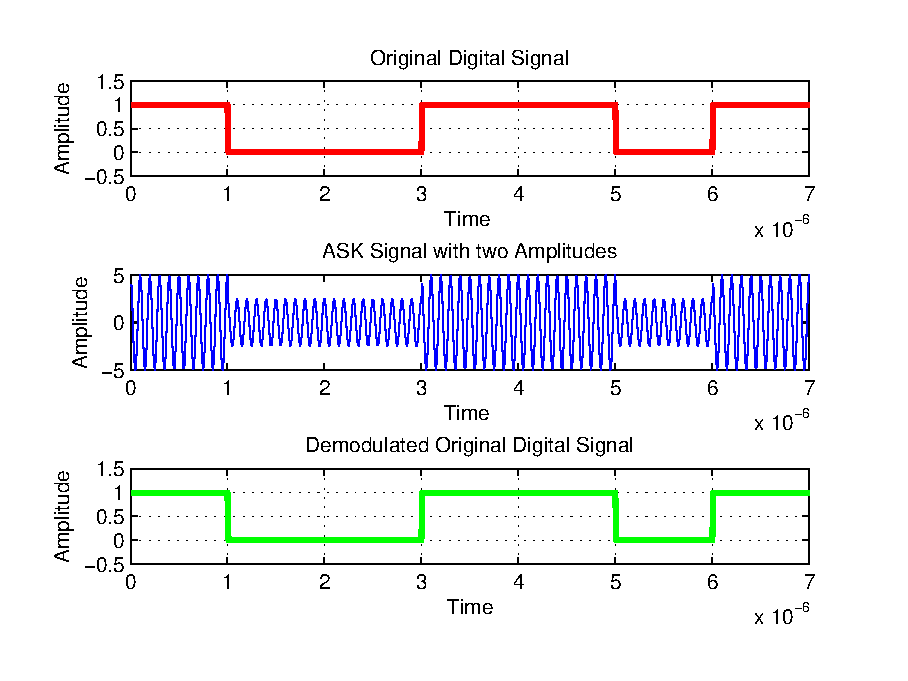
\includegraphics[width=0.7\textwidth]{ASKexample.eps}
    \caption{ASK modulation example in the absence of noise for amplitudes $a_1=2.5$ and $a_2=5$.}
    \label{ask}
\end{figure}

It is important to have an high signal-noise to ratio, especially when the amplitudes are too close so that the demodulator can identify it, since ASK is very sensitive to atmospheric noise, distortions and propagation conditions.  A possible demodulator is shown in figure (\ref{askdem}).

\begin{figure}[h]
  \centering
    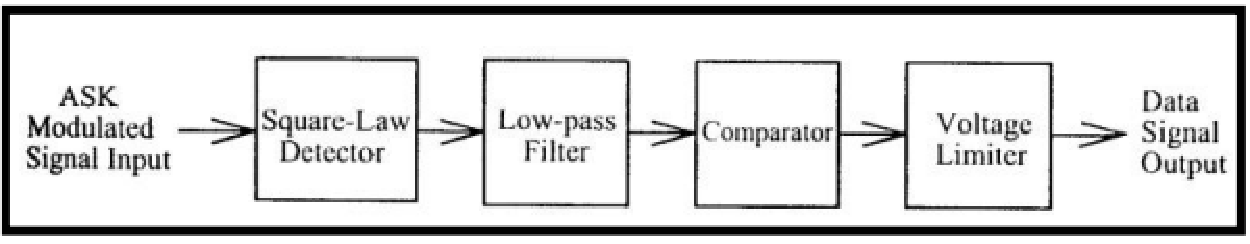
\includegraphics[width=0.7\textwidth]{askdem.pdf}
    \caption{Possible demodulator for ASK.}
    \label{askdem}
\end{figure}

\subsubsection{FSK}
\label{fsk}
Frequency shift keying is a modulation technique where data is transmitted through discrete frequency changes of a carrier wave with fixed amplitude A. The simplest form is the binary FSK (BFSK), where a sine wave $s_i(t)$ is transmitted per bit (as shown in figure(\ref{fskex}). A 0 or 1 is transmitted as a sinusoid of frequency $f_0$ or $f_1$, respectively. 

\begin{figure}[h]
  \centering
    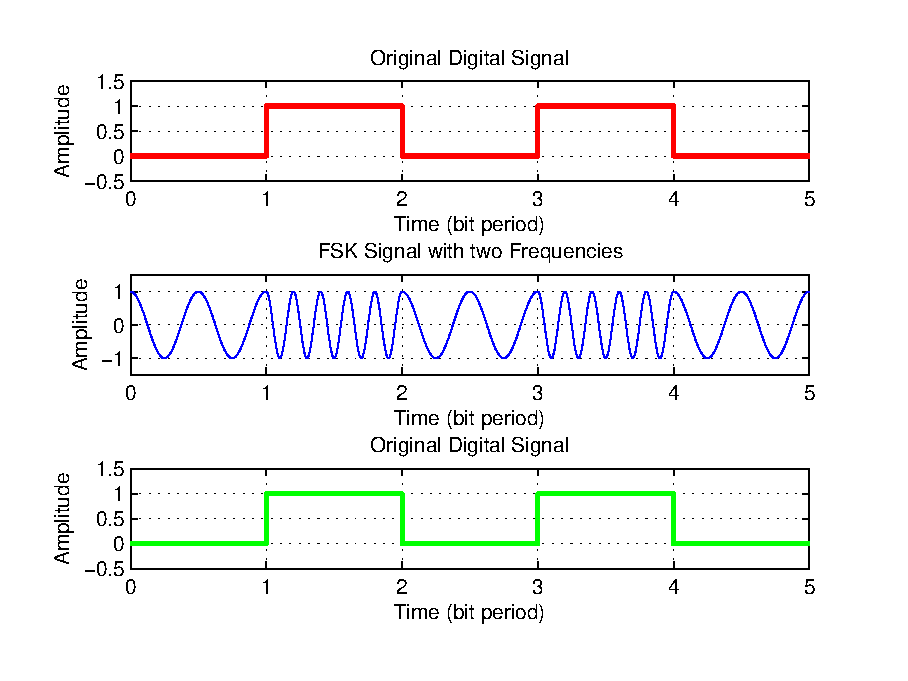
\includegraphics[width=0.7\textwidth]{fskexample.eps}
    \caption{BFSK example for 2 sinusoids of low frequency.}
    \label{fskex}
\end{figure}

Multiple sinusoids of different frequencies can also be used  transmit n bits. In order to guarantee they are orthogonal, there should be $M=2^n$ frequencies separated by $\Delta f=\frac{k}{2T}$, where k is an integer and T is the bit period. The complex baseband signalling waveforms for M-ary FSK are hence given by:

\[{s_i}(t) = {e^{j2\pi {f_i}t}}{I_{[0,T]}},i = 1,2,...,M\]



In terms of demodulation, coherent and noncoherent methods exist and they depend on if the phase of the sinusoids $\phi$ are equal or not. Coherent demodulators consist of correlators or equivalently, matched filters and samples but they require the synchronization of the reference signals. The demodulator for the BFSK can be implemented with two correlators as shown in figure (\ref{coherent}). This receiver is optimum in the sense that it minimizes the error probability for equally likely binary signals. If a sinusoid with frequency $f_1$ is transmitted, for example, the upper correlator yields a signal $l_1$ with positive signal component while $l_2$ has only a noise component, due to signals’ orthogonality.
  In case there is no chance of having a phase reference, then additional squarers or envelope detectors must be used for the noncoherent detection. In the last case a minimum tone spacing of $\frac{k}{T}$ is required instead. The correlator implementation for noncoherent BFSK can be seen in figure (\ref{noncoherent}).

 \begin{figure}[h]
 \centering
\begin{subfigure}[h]{0.9\textwidth}
 \centering
    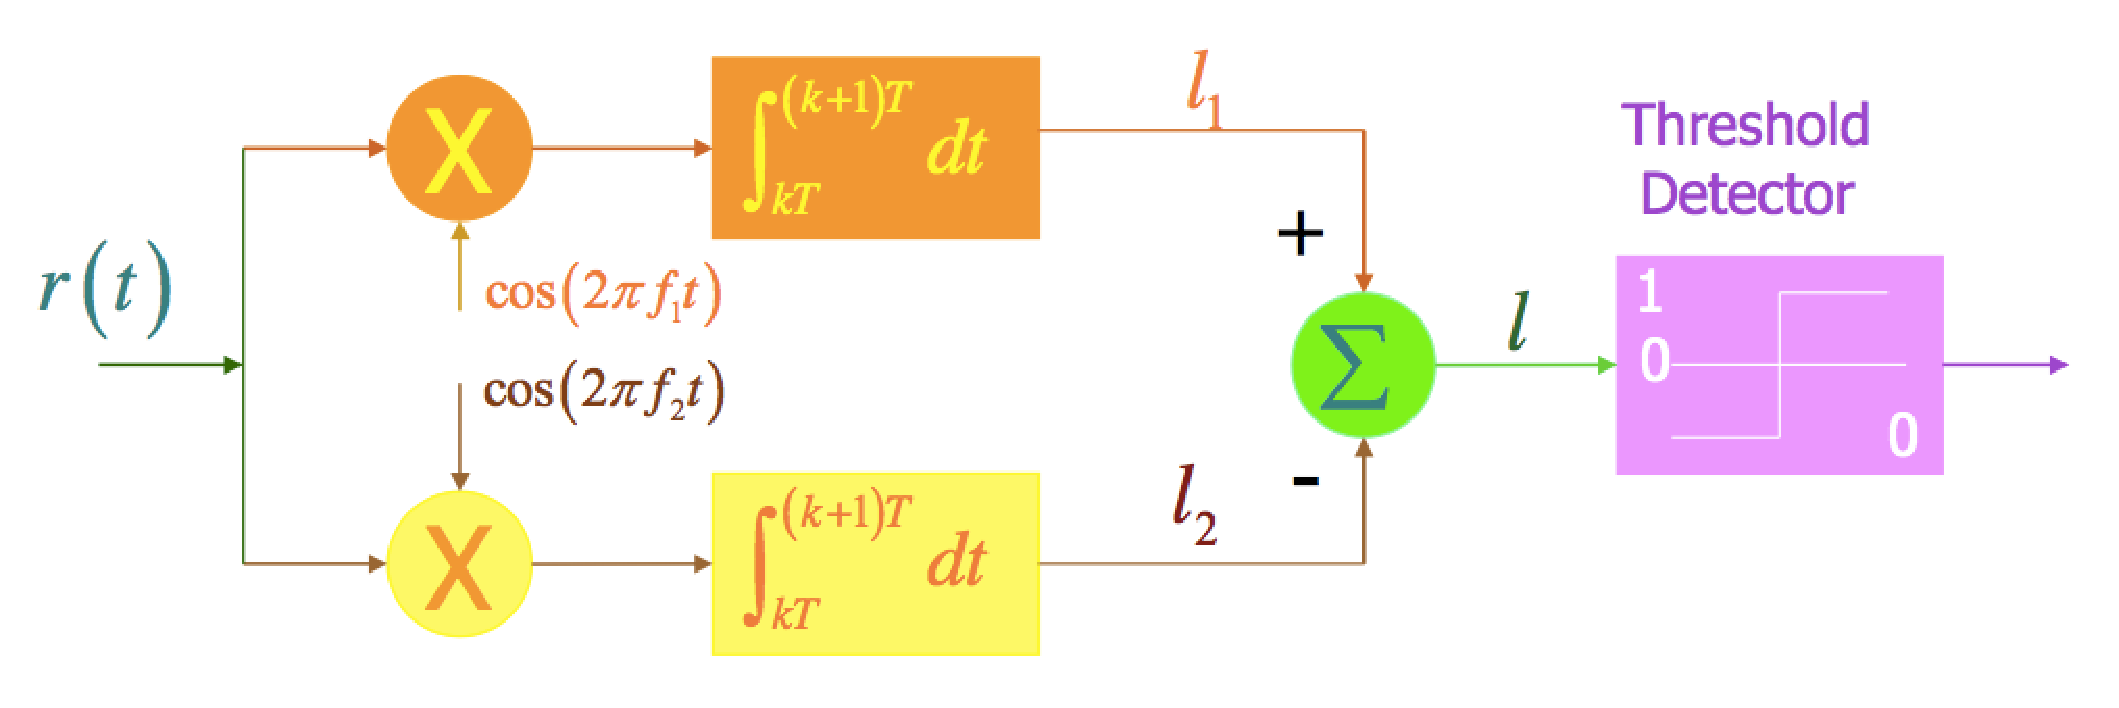
\includegraphics[width=0.6\textwidth]{fskdem1.pdf}
    \subcaption{Coherent.}
    \label{coherent}

\end{subfigure}
\quad

\begin{subfigure}[h]{0.9\textwidth}
 \centering
    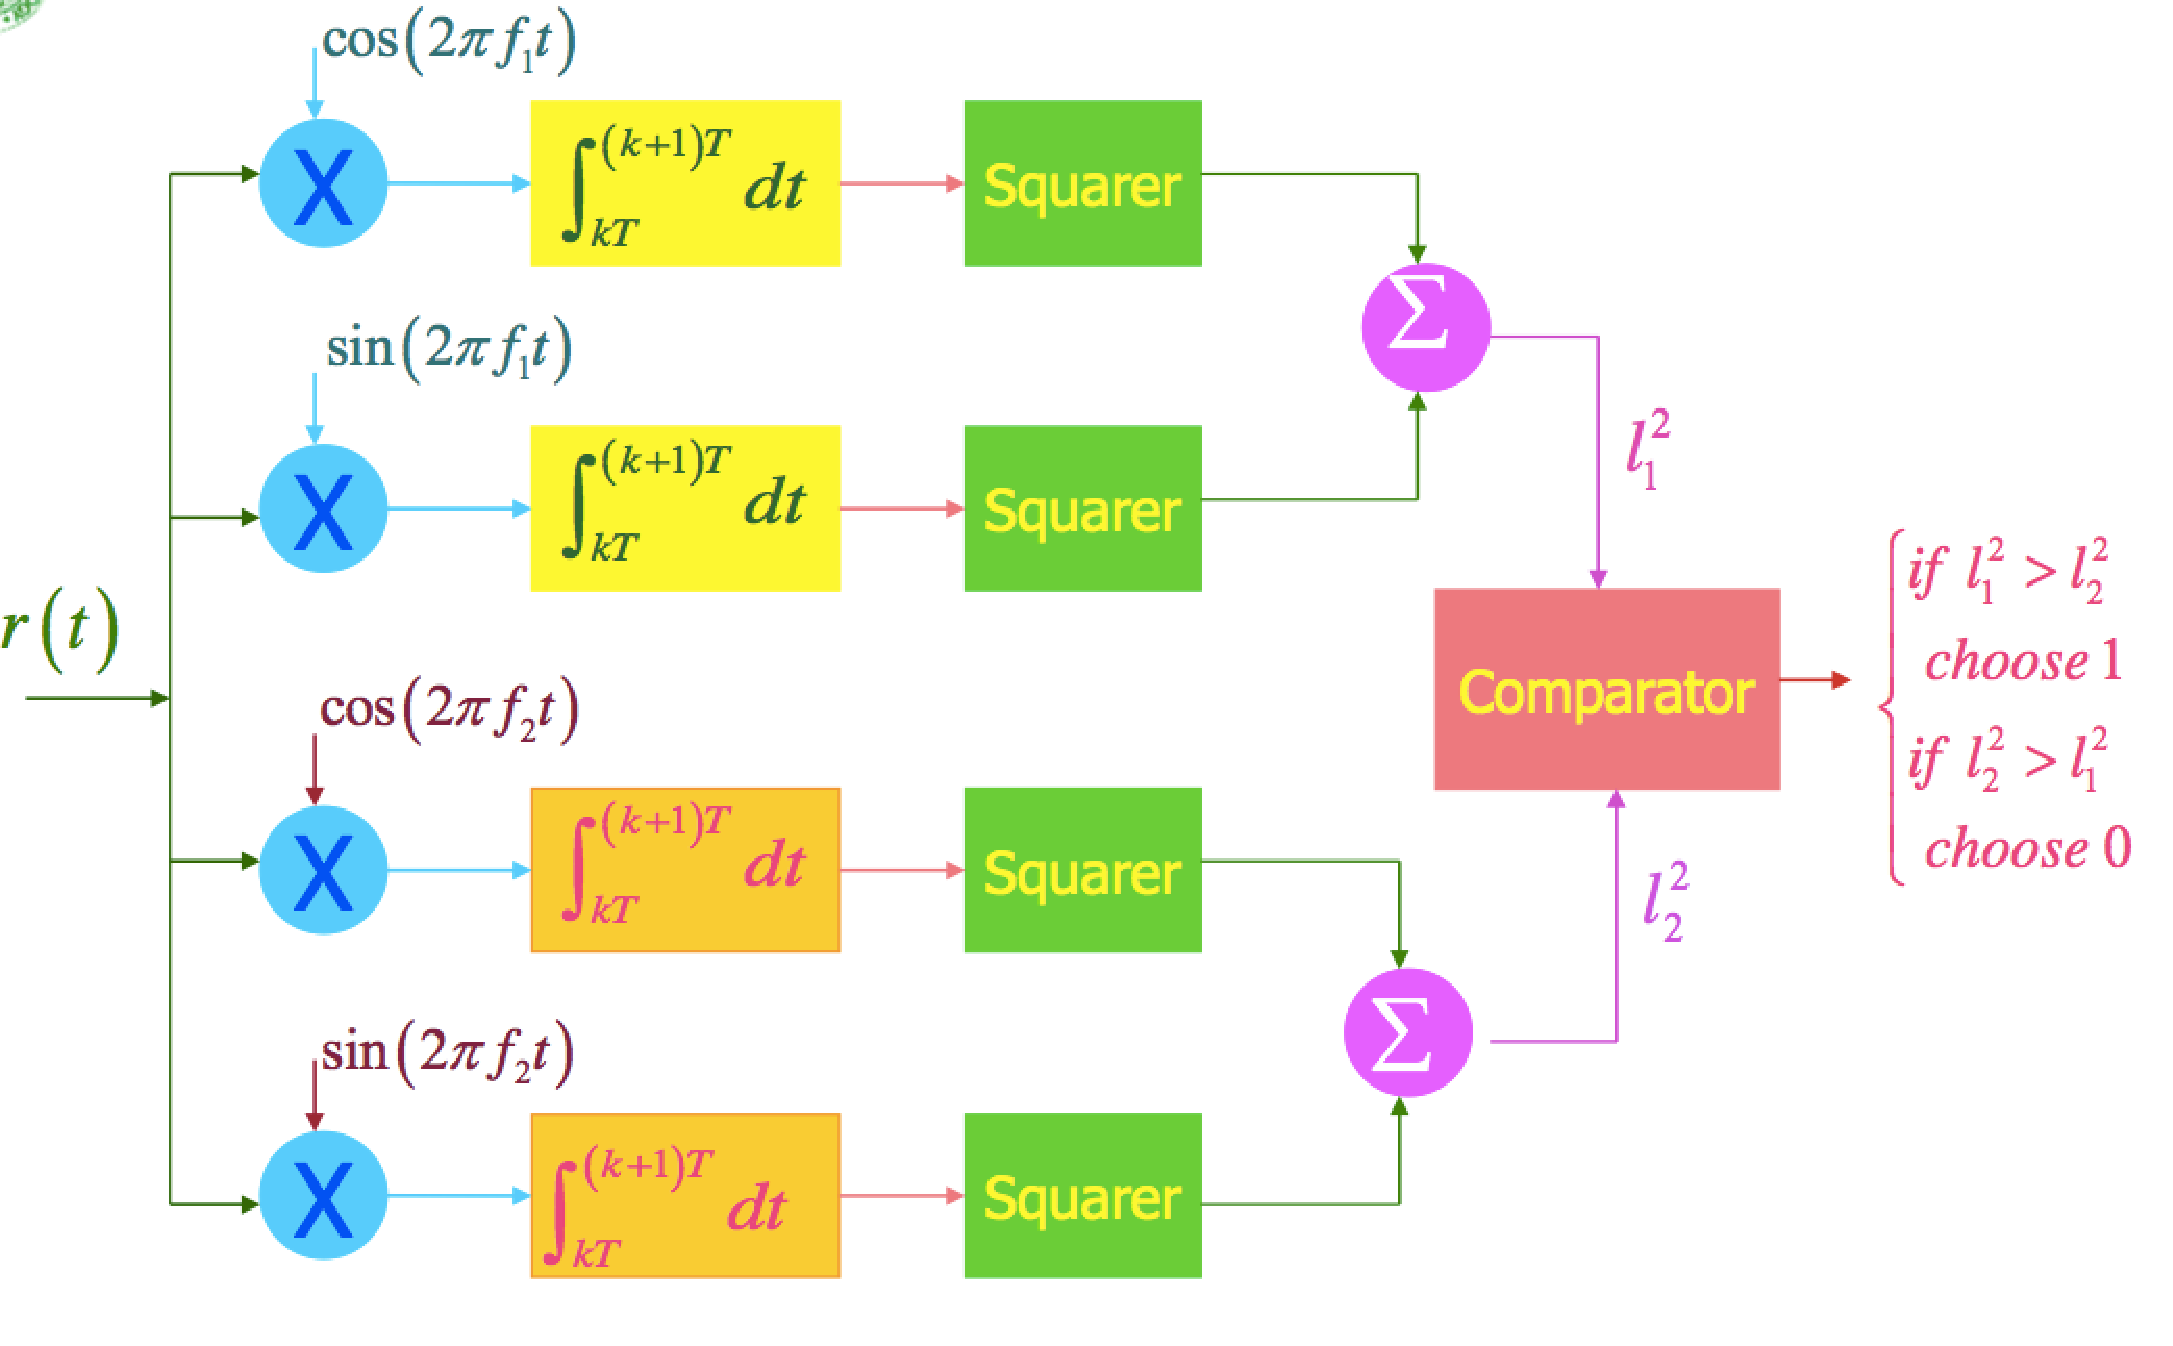
\includegraphics[width=0.6\textwidth]{fskdem2.pdf}
    \subcaption{Non-coherent.}
    \label{noncoherent}
    \end{subfigure}
    \caption{Possible Demodulators for FSK.}
\end{figure}


It is expected that the error performance of the non-coherent receivers is inferior to that of the coherent ones. However, the degradation in only a fraction of dB. Other options for demodulation are available such as the use of FFT schemes for peak picking or bandpass filtering at the used frequencies. 
The main advantages of this modulating scheme are the insensitiveness to amplitude variations in the channel, its compatibility with non-linear transmitter and receiver systems and an absolute frequency accuracy is not a requirement for correct demodulation (making it tolerant to local oscillators drifts and Doppler shifts). The drawbacks are the fact that is less bandwidth efficient when compared with other schemes such as ASK or PSK. To avoid undesirable spectral characteristics which could cause adjacent channel interference, continuous phase FSK is required (for comparison, see figure \ref{comparecpfsk}.

 \begin{figure}[h]
 \centering
\begin{subfigure}[h]{0.9\textwidth}
 \centering
    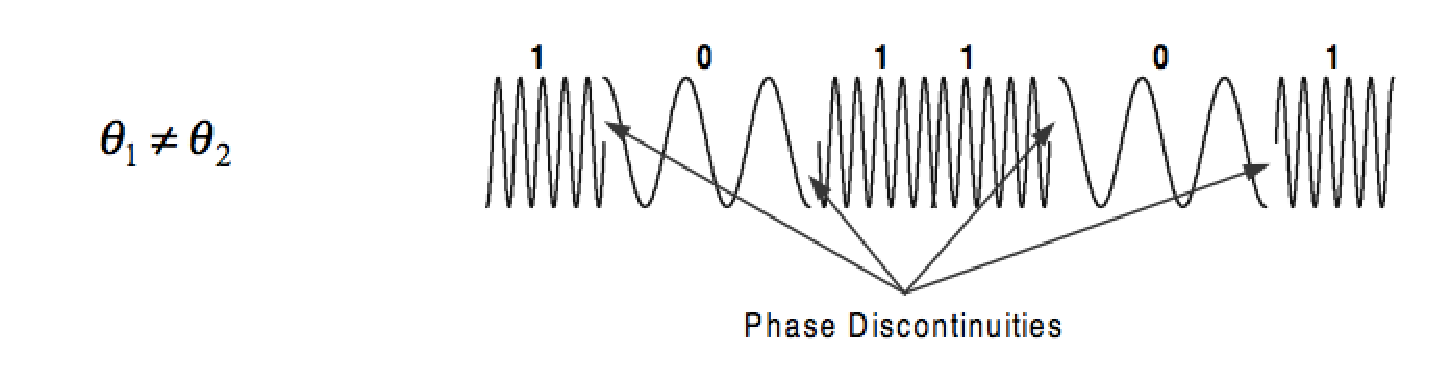
\includegraphics[width=0.6\textwidth]{ncpfsk.pdf}
    \subcaption{Non continuous phase FSK.}
    \label{coherent}

\end{subfigure}
\quad

\begin{subfigure}[h]{0.9\textwidth}
 \centering
    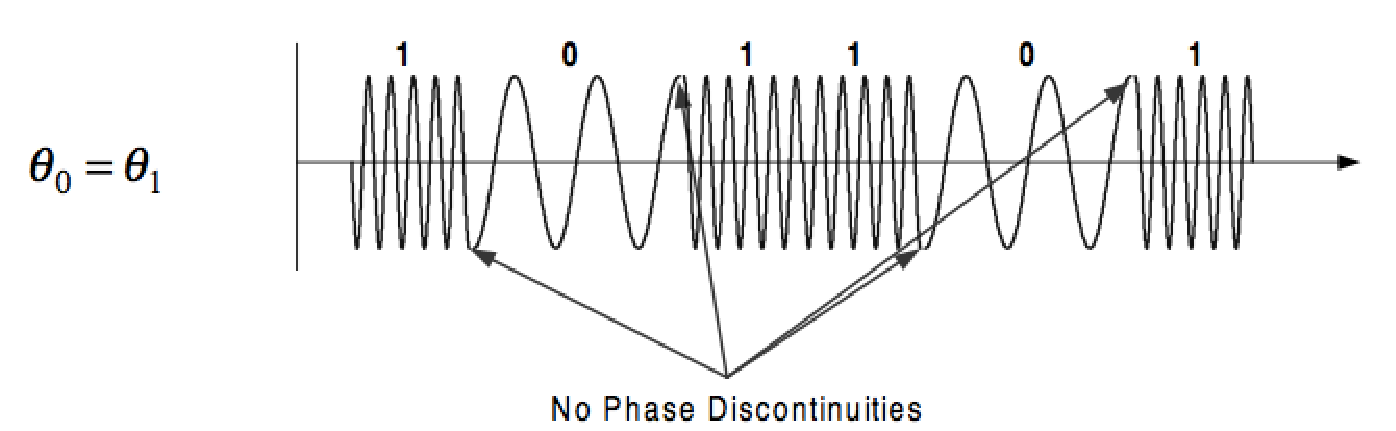
\includegraphics[width=0.6\textwidth]{cpfsk.pdf}
    \subcaption{Continuous phase FSK.}
    \label{noncoherent}
    \end{subfigure}
    \caption{FSK transmitted wave, with and without phase discontinuity.}
    \label{comparecpfsk}
\end{figure}


\subsubsection{PSK}

Phase-shift keying is a digital modulation scheme that conveys data by changing, or modulating, the phase of a reference signal (the carrier wave). A finite number of phases are assigned a unique pattern of binary digits. Usually, each phase encodes an equal number of bits. The demodulator, which is designed specifically for the symbol-set used by the modulator, determines the phase of the received signal and maps it back to the symbol it represents. In digital phase modulation, the M signal waveforms may be represented as: 
\[{s_i}(t) = A\cos ({\omega _c}t + {\phi _i}(t)) = \overbrace {A\cos ({\phi _i}(t))}^{inphase{\rm{ symbol }}{{\rm{x}}_i}(t)}*\cos ({\omega _c}t) + \underbrace {( - A\sin ({\phi _i}(t)))}_{{\rm{quadrature symbol }}{{\rm{x}}_q}(t)}*\sin ({\omega _c}t) = {x_i}(t)\cos ({\omega _c}t) + {x_q}(t)\sin ({\omega _c}t)\]

where $T_s$ is the symbol period, A the amplitude and M the number of points in constelation diagram and the number of phases existing in the system. The decision regions for two different MPSK schemes can be seen in figure \ref{pskdr}.

 Alternatively, instead of using the bit patterns to set the phase of the wave, it can be used to change it by a specified amount. The demodulator then determines the changes in the phase of the received signal rather than the phase itself. Since this scheme depends on the difference between successive phases, it is termed differential phase-shift keying (DPSK). 
 \begin{figure}[h]
  \centering
    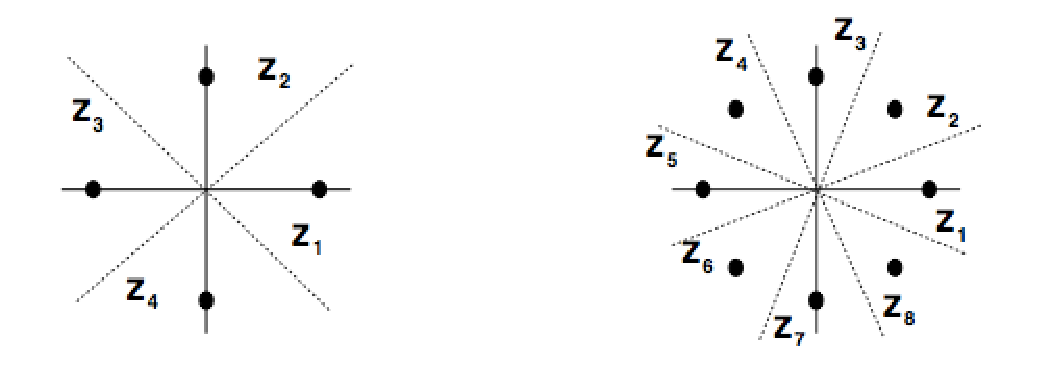
\includegraphics[width=0.7\textwidth]{PSKmodulation.pdf}
    \caption{Decision regions for quadrature and 8-ary PSK. The minimum distance between symbols is given by $d_{min}=A\sin\frac{2\pi}{M}$.}
    \label{pskdr}
\end{figure}

The advantages of PSK/DPSK is a more efficient use of bandwidth when compared with FSK. However, the signal detection/recovery is much harder when compared with ASK and FSK since the demodulator must determine the phase of received sinusoid with respect to some reference phase. Additionally if a higher rate PSK scheme is used the equipment must be able to distinguish small differences in phase, making it unusable in time-varying channels. 


\section{Method}

In the last section, the fundamentals of each modulation scheme were introduced. Now we will focus on developing the details of the implemented modulation, demodulation and coding schemes. 

\subsection{MFSK}

FSK systems enjoy the highest power efficiencies among the available modulation schemes but are accompanied by the lowest bandwidth (BW) efficiency. In the following lines, we purpose a scheme of using M-ary FSK system modulation with orthogonal envelopes to improve BW efficiency of MFSK modulation. In M-ary FSK schemes, the modulated signals can be represented by:

\[{s_m}(t) = A{\varphi _m}(t),0 \le t \le T\],

where $T_s$ is the period of the input symbol stream and A the amplitude of the basis function $\varphi_m$. This basis function can be described by:

\[{\varphi _m}(t) = \sqrt {\frac{2}{T}} \cos \left( {2\pi ({f_c} + {\alpha _m}\Delta {f_c}) + {\theta _m}} \right),0 \le t \le T\]


where \[{\alpha _m} \in \left\{ {(2m - 1 - M)|m = 1,2,...,M} \right\}\]. For orthogonality of the signals, the inner product between the basis functions must be 1 for $m=n$ and 0 for $m\neq n$, that is: 

\[\left\langle {\left. {{\varphi _m},{\varphi _n}} \right\rangle } \right. = \int {{\varphi _m}(t){\varphi _n}(t)dt = {\delta _{mn}} = \left\{ \begin{array}{l}
1,m = n\\
0,m \ne n
\end{array} \right.} \]


Individual frequencies corresponding to different symbols are given by \[{f_m} = {f_c} + {\alpha _m}\Delta {f_c}\], where $f_c$ is the central frequency and $\Delta f_c$ the frequency separation. In order to keep orthogonality, we must have \cite{gold}:

\[\Delta {f}= 2\Delta {f_c} = \left\{ \begin{array}{l}
\frac{1}{{2T}},{\theta _m} = {\theta _n},\forall m,n\\
\frac{1}{T},{\theta _m} \ne {\theta _n}
\end{array} \right.\]

The overall bandwidth occupied by the FSK signal depends on the modulation index $h=\frac{2\Delta {f_c}}{R}=2\Delta {f_c}T_s$ and for continuous phase BFSK the minimum value for the signals to not interfere with each other is $h=0.5$. Moreover, an FSK system using continuous phase transitions will have much lower side-lobe energy than the discontinuous case. All these parameters will hence affect the ISI and limit the rate of the system. It is then important to further increase the bandwidth efficiency of the system by applying a pulse shaping function to the transmitted signal.

\subsection{Pulse Shaping Functions}

So far, we were considering the case where the signal is shaped by a rectangular function, inside the interval $0\leq t \leq T_s$. If g(t), the pulse shaping function, is a rectangular pulse of width of $T_s$, then the envelope of the signal is constant. However, a rectangular pulse has very high spectral sidelobes, which means that signals must use a larger bandwidth to eliminate some of the adjacent channel sidelobe energy. Pulse shaping is a method to reduce sidelobe energy relative to a rectangular pulse, however the shaping must be done in such a way that intersymbol interference (ISI) between pulses in the received signals is not introduced (or, at least, minimised). Assuming the channel model to be AWGN, the effective receive pulse is given by $p(t)=g(t) \ast c(t) \ast g^{*}(-t)=g(t) \ast g^{*}(-t)$, since the channel impulse response is given by $c(t)=\delta(t)$. This pulse must satisfy the Nyquist criterion, which requires the pulse to equal zero at the ideal sampling point associated with past or future symbols: 

 \[p(k{T_s}) = \left\{ \begin{array}{l}
{p_0} = p(0),k = 0\\
0,k \ne 0
\end{array} \right.\]

Some of the pulses that satisfy this criterion are the rectangular, cosine and raised cosine. Each pulse has its advantages and disadvantages and aim to improve spectral efficiency but a mistiming error in sampling leads to a series of ISI components that converge. The most common pulse shape in FSK is the Gaussian pulse shape defined as: 

\[g(t) = \frac{{\sqrt \pi  }}{\alpha }{e^{ - {\pi ^2}{t^2}/{\alpha ^2}}}\]

where $\alpha$ is a parameter that dictates spectral efficiency. The spectrum of g(t) is is given by: 
\[G(f) = {e^{ - {\alpha ^2}{f^2}}}\]


The different windows characteristics can be seen in figure \ref{wc} and their effect when applied to a simple BFSK system in figure \ref{wcomp}. The parameter $\alpha$ in the gaussian window is related to the 3dB bandwidth of g(t), $B_z$:
\[\alpha  = \frac{{\sqrt { - \ln \sqrt {0.5} } }}{{{B_z}}}\]

 \begin{figure}[h]
 \centering
  \label{wincar}
\begin{subfigure}[h]{1\textwidth}
 \centering
    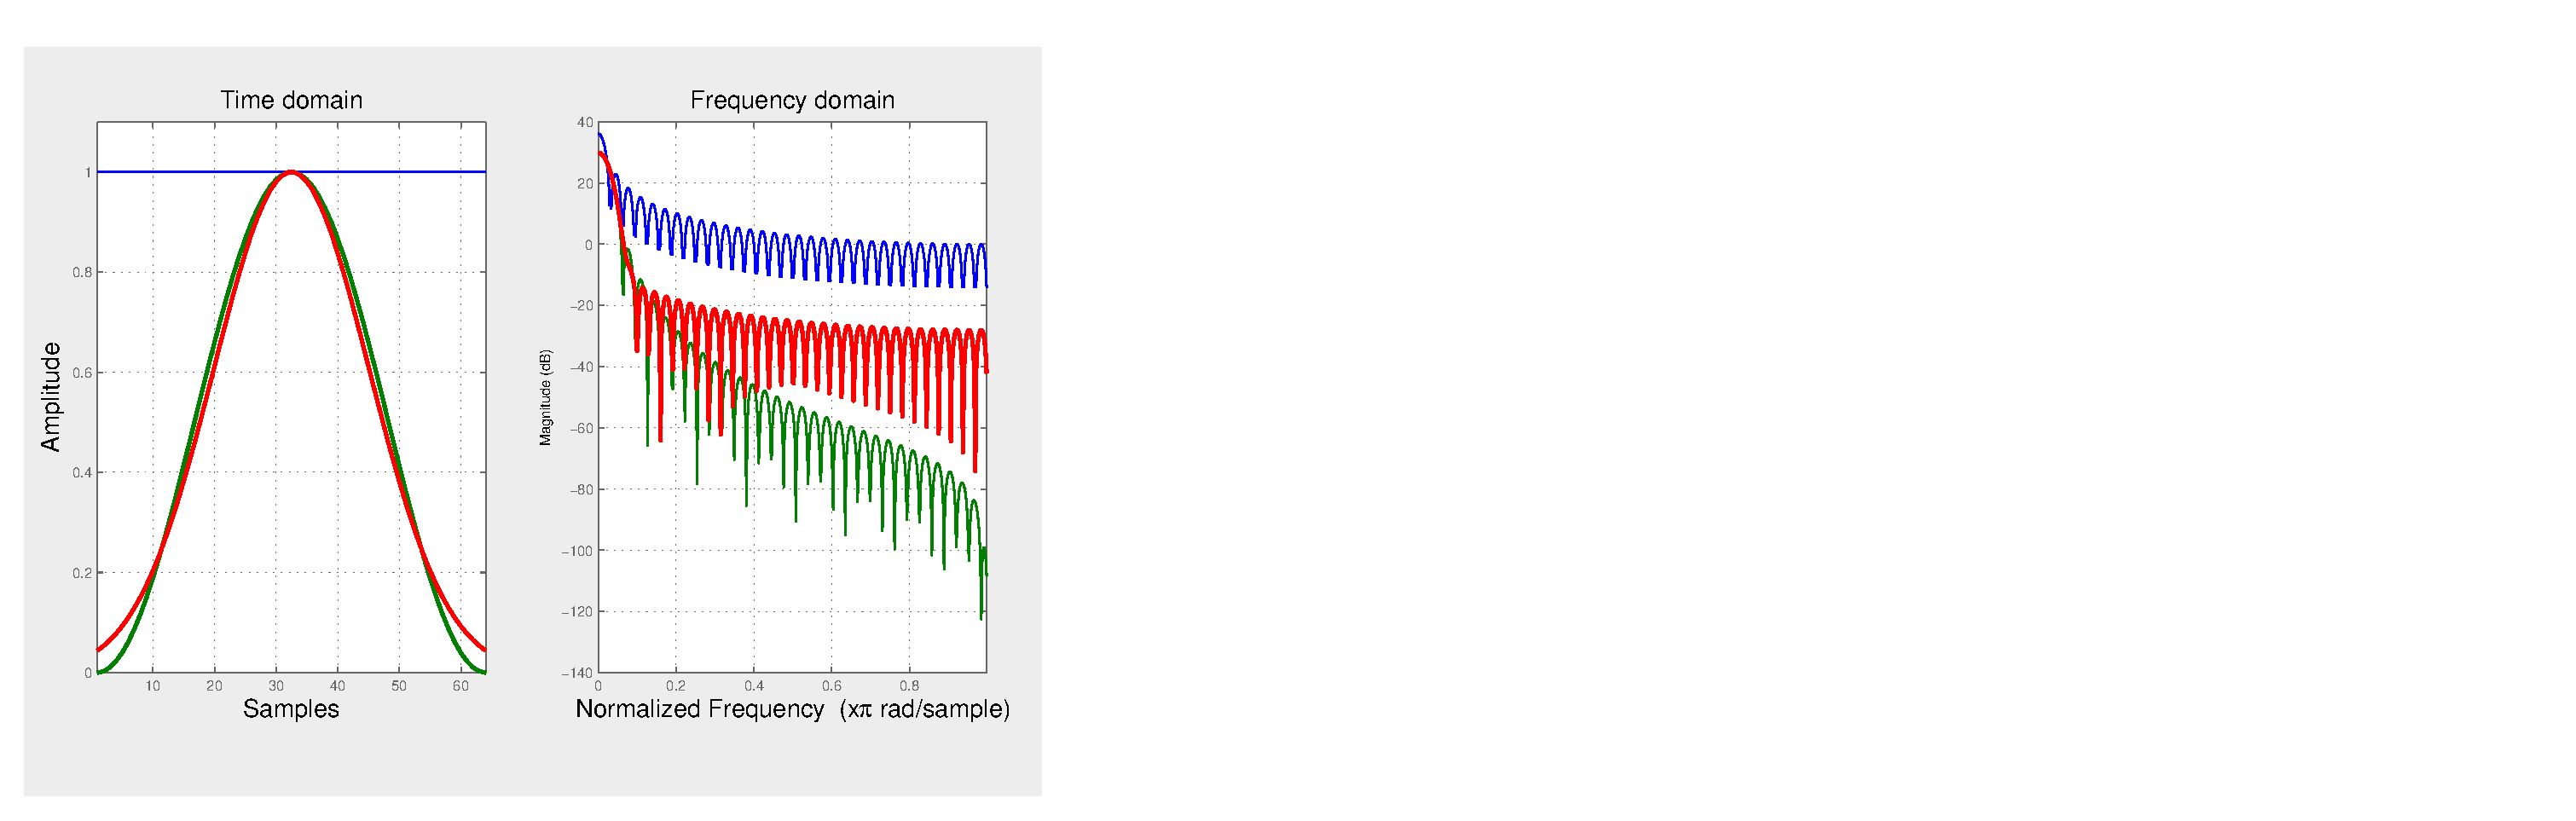
\includegraphics[scale=0.45, trim=0 0 30cm 0, clip=true]{wincomp.eps}
    \subcaption{Different windows in time and frequency domain. \textbf{Blue, red and green lines correspond to the rectangular, Gaussian and Hanning window, respectively.}}
    \label{wc}
\end{subfigure}

\qquad
\qquad

\begin{subfigure}[h]{1\textwidth}
 \centering
    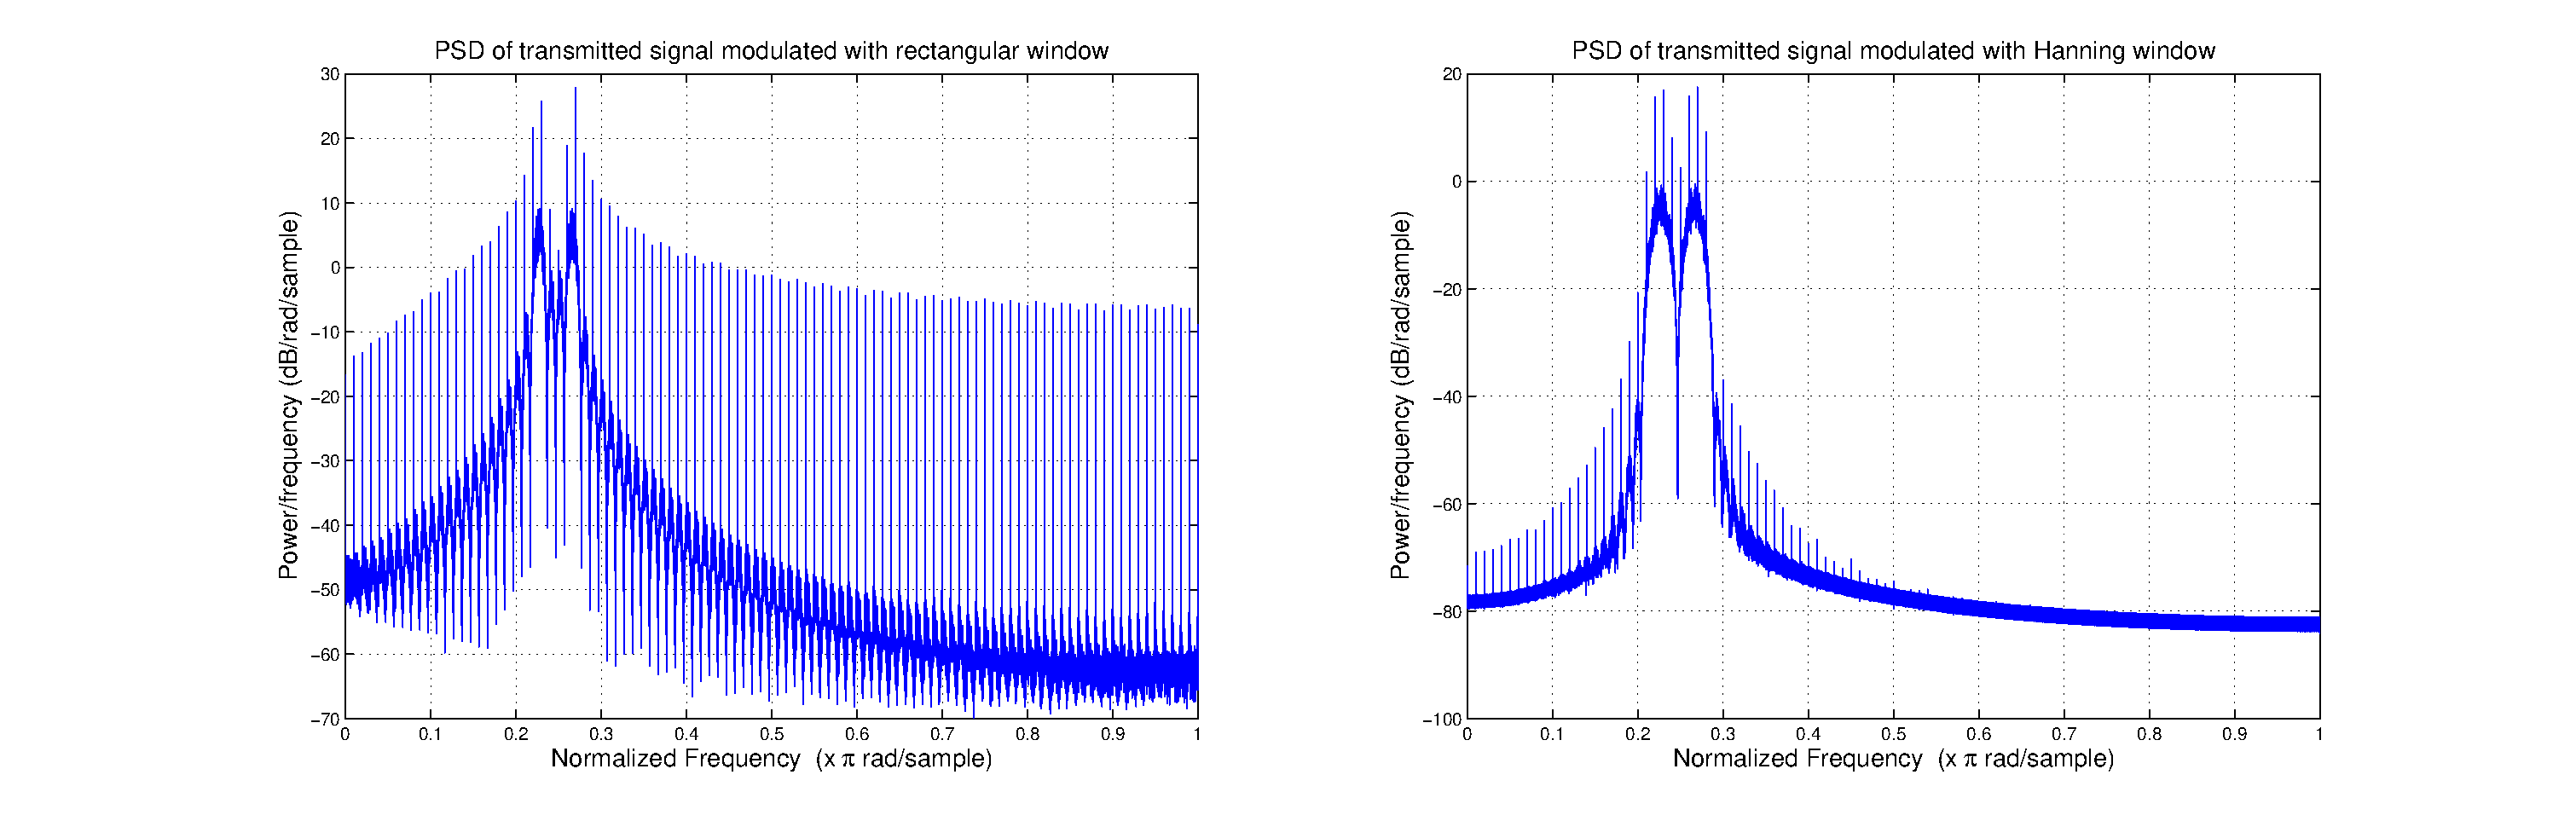
\includegraphics[scale=0.38]{txwinrectVShann.eps}
    \subcaption{PSD of the transmitted pulse using the rectangular and Hanning window for a BFSK system.}
    \label{wcomp}
    
    \end{subfigure}
    
    \caption{The importance of choosing the right window for pulse shaping.}
    \label{main}
\end{figure}

 Obviously, making $\alpha$ large results in a higher spectral efficiency. The Gaussian pulse does not satisfy the Nyquist criterion, and therefore the pulse shape introduces ISI, which increases as $\alpha$ increases. Therefore, improving spectral efficiency by increasing $\alpha$ leads to a higher ISI level, thereby creating an irreducible error floor from this self-interference. The variable $\alpha$ should, hence, be chosen with care. The gaussian window effect can be seen in figure \ref{gaussianalpha} and will be further developed in the training sequence section \ref{ts}.

 \begin{figure}[h]
  \centering
    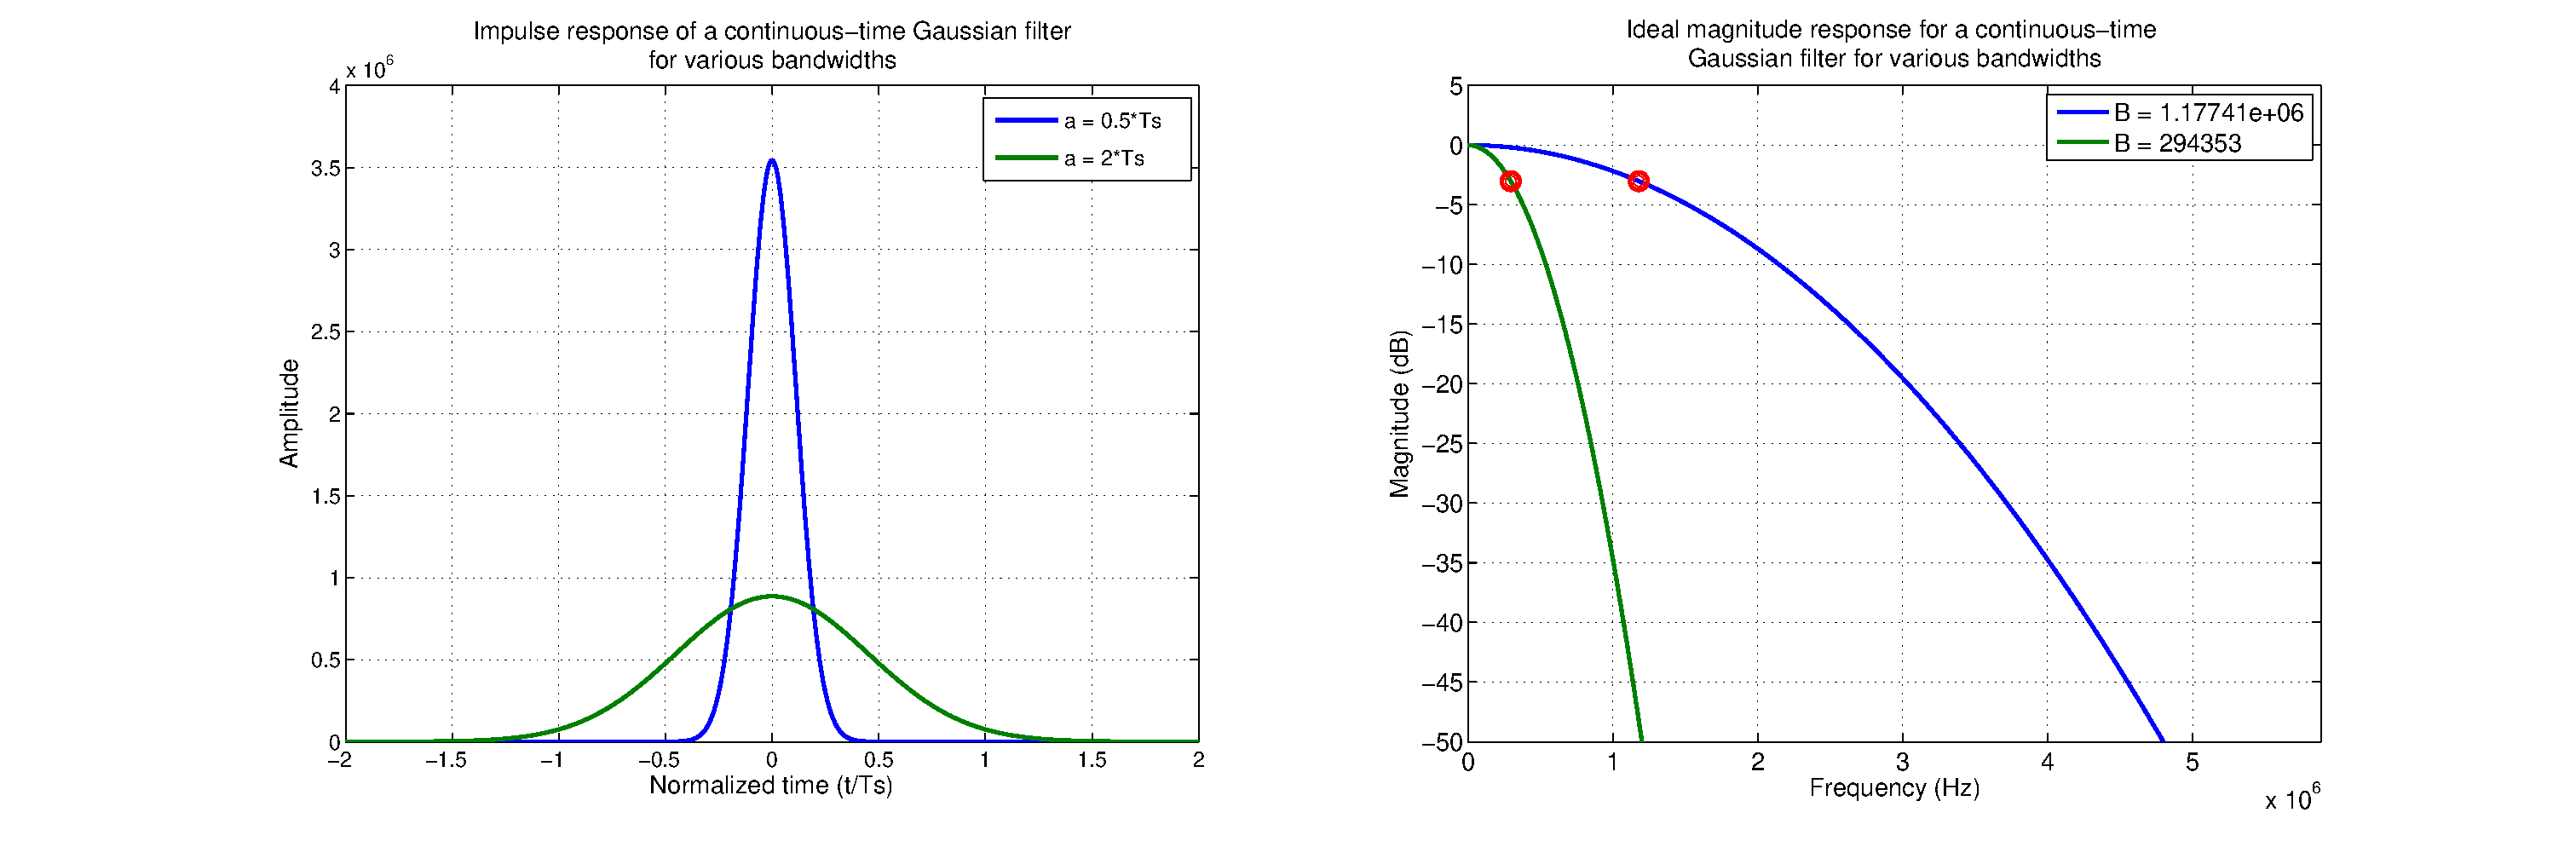
\includegraphics[width=1\textwidth]{gausswinalpha.eps}
    \caption{Ideal Gaussian filter with different values of $\alpha$. The tradeoff between high spectral efficiency and reduced ISI is clear. A large $\alpha$ leads to an increased efficiency but the amplitude for $t/T_s > 1$ is not zero, leading to ISI.}
    \label{gaussianalpha}
\end{figure} 
 

\subsection{Efficient MFSK Demodulation}

The demodulators presented in part \ref{fsk} are interesting from a theory point of view. However, for real time, software based applications there exist other methods for efficient demodulation. One of these methods is the Discrete Fourier Transform (DFT) which evaluates the amplitude and phase for each frequency present in the received signal. Since we are using a MFSK modulation scheme, a tone/frequency detector such as DFT for a symbol period is a powerful tool for correct efficient demodulation. However, we are only interested in detecting one or more tones in an audio signal and at the same time we are constrained to the CPU horsepower provided by the smartphone. Taking this into account, we purpose a much faster method, when compared with FFT for instance, which is the Goertzel algorithm. 

\subsection{Goertzel Algorithm}

There are various to detect the presence of a special known frequency in a received signal. The DFT algorithm is a simplistic way to check whether the desired frequency is present and a FFT produces the same numerical result for a single frequency of interest, making it a better choice for tone detection. The Goertzel algorithm is a DFT in disguise, with some numerical tricks to eliminate complex number arithmetic, increasing the efficiency over the FFT under some constraints. This section aims to present the Goertzel algorithm.

The idea is to transform an ordinary N samples DFT into a Goertzel filter form. Defining $W_{N}^{k}={e^{ - j2\pi k/N}}$, noting that ${W_N}^{ - Nk} = 1$, we have for the DFT:
\[X(k) = \sum\limits_{n = 0}^{N - 1} {x(n){W^{nk}}_N}  = \sum\limits_{n = 0}^{N - 1} {x(n){W_N}^{ - Nk}{W^{nk}}_N}  = \sum\limits_{n = 0}^{N - 1} {x(n){W_N}^{ - (N - n)k}} \]
An efficient way to evaluate this polynomial is the nested form:
\[X(k)=\bigg(\big(({W^{ - k}_N}x(0) + x(1)\big){W_N}^{ - k} + x(2)){W_N}^{ - k} + ... + x(N - 1)\bigg){W_N}^{ - k}\]

The last expression can be written in terms of a recursive difference equation:
\[y(n) = {W^{ - k}_N}y(n - 1) + x(n)\]

Expressing the difference equation as z-transform and multiplying both numerator and denominator by gives the transfer function:

\[\frac{{Y(z)}}{{X(z)}} = H(z) = \frac{1}{{1 - {W_N}^{ - k}{z^{ - 1}}}} = \frac{{1 - {W_N}^{ - k}{z^{ - 1}}}}{{1 - (2\cos (\frac{{2\pi k}}{N}){z^{ - 1}} - {z^{ - 2}})}}\]

The Goertzel algorithm acts as an IIR filter that uses the feedback path to generate a very high Q bandpass filter where the coefficients are easily generated from the required center frequency.  It is mostly implemented as the second order recursive IIR filter as shown in figure \ref{IIR}. 
 \begin{figure}[h]
  \centering
    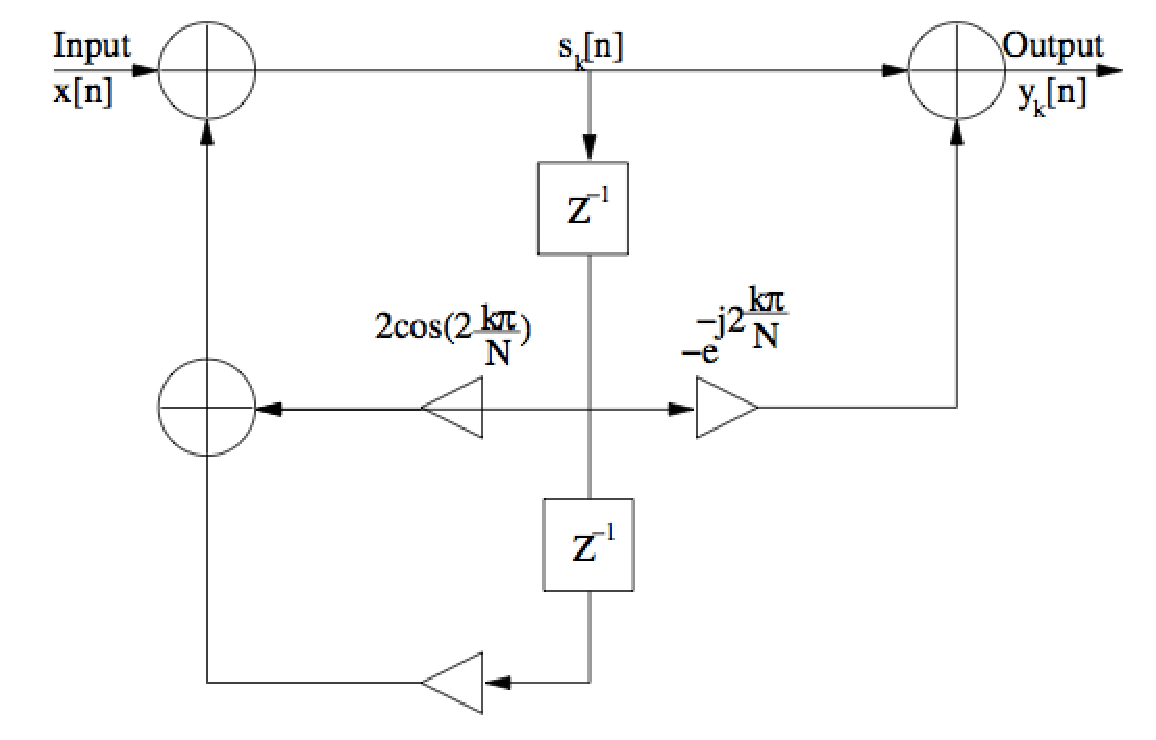
\includegraphics[width=0.5\textwidth]{IIR.pdf}
    \caption{Direct-Form Realisation of the Goertzel Algorithm.}
    \label{IIR}
\end{figure}


The algorithm computes the k-th DFT coefficient X(k)=y(N) of the input signal $x(n)$ using the 2nd order filter:
\begin{equation}
\begin{array}{l}
{s_k}(n) = x(n) + 2\cos (\frac{{2k\pi }}{N}){s_k}(n - 1) - {s_k}(n - 2)\\
{y_k}(n) = {s_k}(n) - {W_N}^k{s_k}(n - 1)
\end{array}
\label{IIRtime}
\end{equation}

with ${s_k}( - 1) = {s_k}( - 2) = 0$. The discrete frequencies where the algorithm is able to compute the DFT are ${f_k} = \frac{k}{N}{f_s}$ for $f \leq \frac{f_s}{2}$.
%%The computation for $s_k(n)$ takes one add ($x(n)-s_k(n-1)$) and one %%multiply-accumulate per received sample.

\subsubsection{Computational and Memory complexities}

The FFT algorithm used with N being a power of two has computational demands proportional to $\mathcal{O}(N\log_2 N)$, the absolute number depends on the particular implementation. Usually the number of real-number operations found in the literature is approximately $6N \log_2 N$. If we analyze the number of operations of the Goertzel algorithm, we realize that for a real input signal, $N$ real multiplications and $2N$ real additions are performed and, hence, $3N$ operations for a single frequency. Ignoring the computations of the cosine and the exponential constants in equation \ref{IIRtime}, then if N frequencies would be of interest, the Goertzel algorithm would be of quadratic complexity as the DFT is. To answer the question for how many frequencies K is it more advantageous to exploit the Goertzel algorithm than the FFT we compare and conclude that: 
\begin{equation}
3NK < 6N{\log _2}N \Leftrightarrow K < 2{\log _2}N
\label{ineffgor}
\end{equation}

Such a result, however, holds only for N being a power of two; otherwise the inequality \ref{ineffgor} can even be more favourable for the Goertzel algorithm.

Considering real inputs solely, the FFT algorithm requires a memory space of at least 2N. Also the n values of the transformation kernel, sin and cos, are often precomputed and stored. The FFT calculation itself can be performed with no values being moved in memory but as the computation cannot be done until the last sample of a block of data is received, a buffer of at least N in size must be used. Therefore, the overall FFT memory demand is 4N for real signals.
For each considered frequency, the Goertzel algorithm requires: location for saving one real and one complex state variable, the complex final output and the last 2 real outputs $s_k(n) and s_k(n-1)$. There is no need to implement input buffering, because the computation can be run as the new signal samples arrive. The total memory complexity of the Goertzel algorithm is thus $7K$ positions. Combining all the above together, the Goertzel algorithm will be less memory-demanding than the FFT if
\[7K < 4N \Leftrightarrow K < \frac{4}{7}N\]

As long as $N\geq 13$ equation \ref{ineffgor} is decisive for choosing the best algorithm since for these N it holds that $\frac{4}{7} N \leq 2 \log_2 N$.

\subsection{Synchronisation}
\label{ts}
Up to this point we have assumed that the receiver is perfectly synchronised with the transmitter and the only channel impairment is AWGN. In practice, however, it is often found that there is also uncertainty due to the randomness of certain signal parameters caused by distortion in the transmission medium. Perhaps the most common random signal parameter is the carrier phase, which is especially true for narrowband signals. 

In the reception of a digitally modulated signal there are two basic modes of synchronisation:
\begin{enumerate}
\item \textbf{Carrier Synchronisation}  When coherent detection is used in signalling via the modulation of a sinusoidal carrier, knowledge of both frequency and phase of the carrier is necessary. The process of estimating the carrier phase and frequency is called carrier recovery. 

\item \textbf{Clock recovery} To perform demodulation, the receiver has to know the instants of time that at which the modulation in the transmitter changes its state. In other words, the receiver has to know the starting and finishing point of the individual symbols, so that it may determine when to sample. The estimation of these times is called symbol synchronisation.
\end{enumerate}

 

\subsubsection{Symbol Synchronisation}
The synchronisation algorithm is crucial for the operation of the system. Its task is to find the best sampling time for the sampling device. Ideally the MF should be sampled such that the SNR for the decision variable is maximised. For a rectangular pulse shape, the best sampling time $t_{samp}$ is at the peaks coming out from the matched filter (see figure \ref{mfpeaks}).

 \begin{figure}[h]
  \centering
    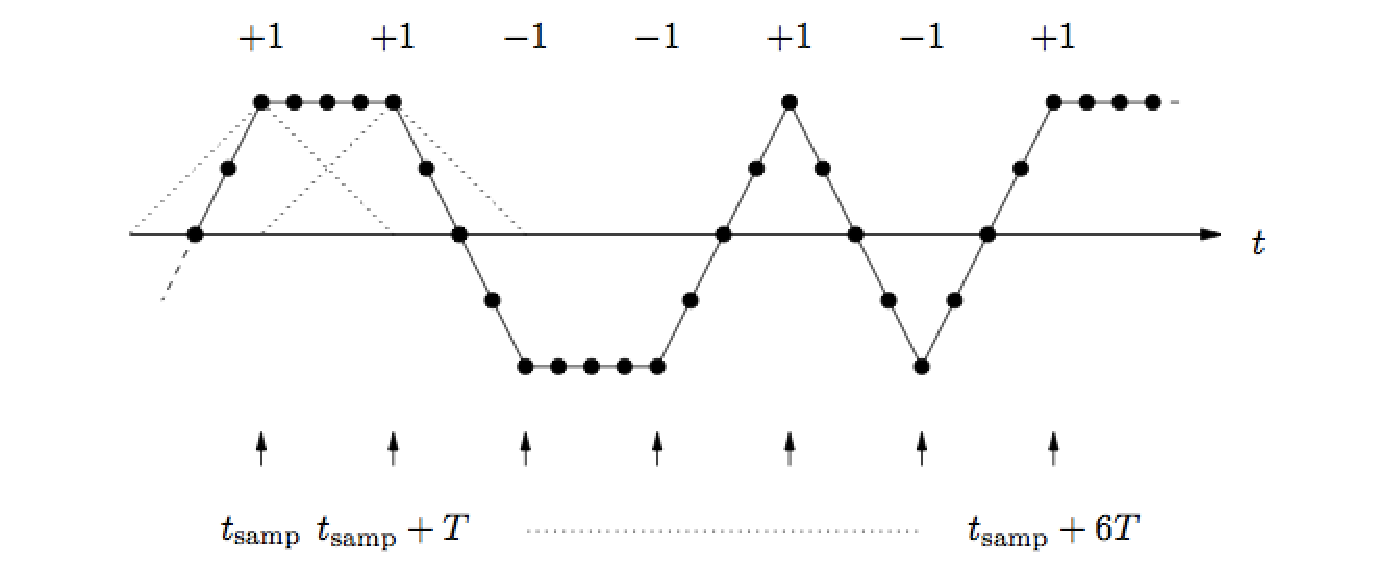
\includegraphics[width=0.7\textwidth]{mfpeaks.pdf}
    \caption{Output from the matched filter for successive signalling in absence of noise. The small arrows illustrate the preferred sampling instants.}
    \label{mfpeaks}
\end{figure}


The used algorithm is based on the training sequence. During the training sequence, it is know to the receiver what the transmitter is transmitting. Hence, one possible way of recovering the symbol time is to cross-correlate the samples after the matched filter with a locally generated time-shifted replica of the training sequence. This algorithm can be either applied directly to the received samples and correlating with a modulated training sequence (resolution of 1 sample but very sensitive) or applied at the symbol level (resolution of $\frac{T}{Q}$, where Q is the number of samples per symbol). Let's consider the last option for simplifying purposes. If ${\left\{ {c(n)} \right\}_{n = 0}^{L - 1}}$ is the locally generated symbol-spaced replica of the training sequence of length L, [$t_{start},t_{end}$] represents the search window and $r(n)$ denotes the output from the matched filter, the timing can be found as:

\[{t_{samp}} = \arg \mathop {\max }\limits_{{t_{samp}} \in [{t_{start}},{t_{end}}]} \left| {\sum\limits_{k = 0}^{L - 1} {r(kQ + {t_{samp}})^*c(k)} } \right|\]


The correlation properties of the training sequence are important as they affect the estimation accuracy. Ideally, the autocorrelation function for the training sequence should equal a delta pulse, i.e., zero correlation everywhere except at lag zero. Therefore, the training sequence should be carefully designed. If, for example, the training sequence is modulated with a different frequency or a different pulse shape is used, from the rest of the signal, better results for the correlation are obtained, as can be seen in figure \ref{tscomp}. 

\begin{figure}[h] 
  \begin{subfigure}[b]{0.5\linewidth}
    \centering
    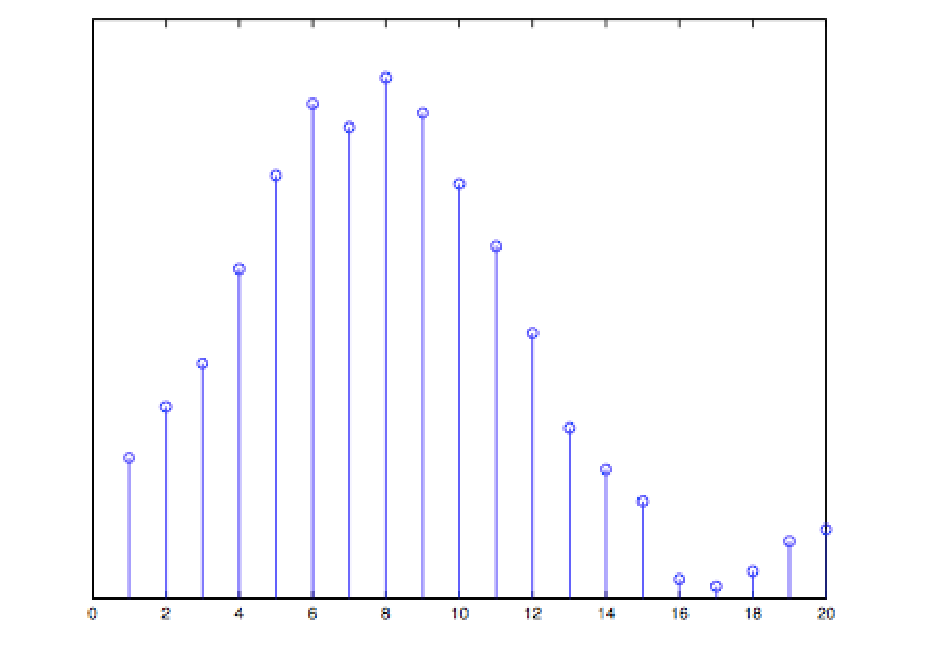
\includegraphics[width=1\linewidth]{ss.pdf} 
    \caption{Symbol spaced cross-correlation. In this example the delay is estimated to be 8 and therefore the system should be sampled at 8+kQ, k=0,1,2,..N.} 
    \label{a} 
    \vspace{4ex}
  \end{subfigure}%% 
  \quad
  \begin{subfigure}[b]{0.5\linewidth}
    \centering
    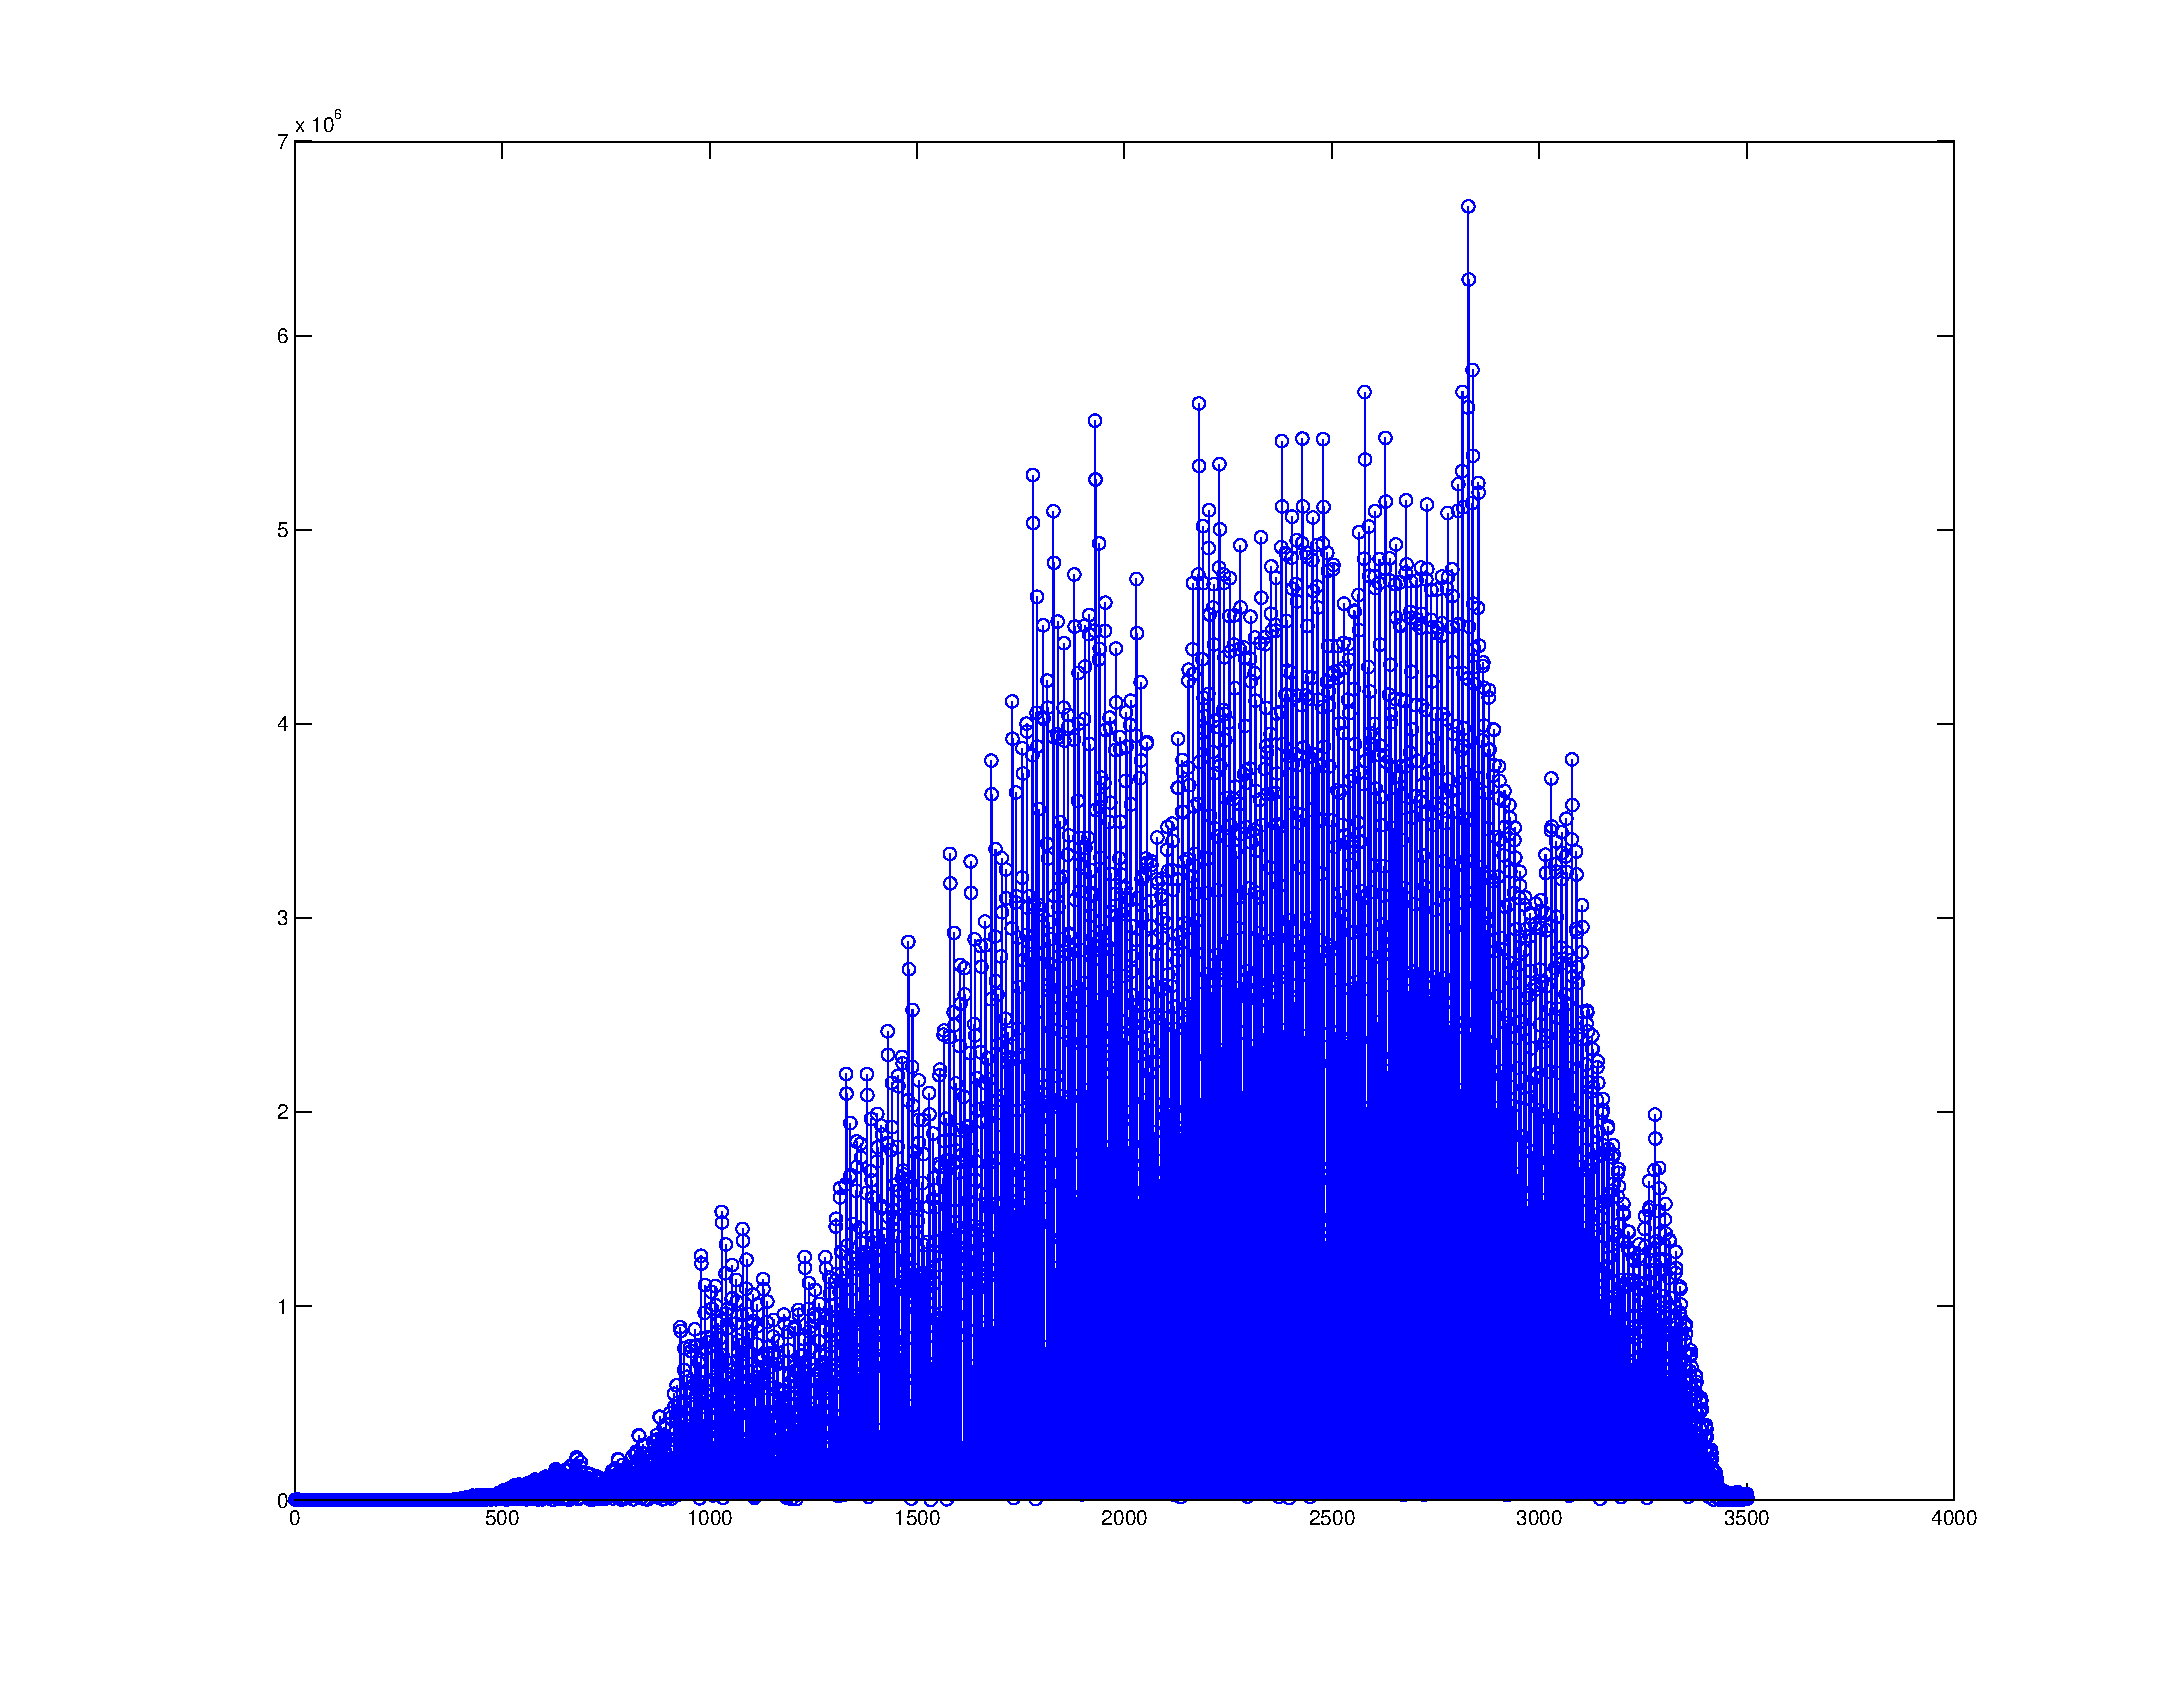
\includegraphics[width=1\linewidth]{20.eps} 
    \caption{One sample resolution cross correlation with training sequence of length 20 symbols.} 
    \label{fig7:b} 
    \vspace{4ex}
  \end{subfigure} 
  \quad
  \begin{subfigure}[b]{0.5\linewidth}
    \centering
    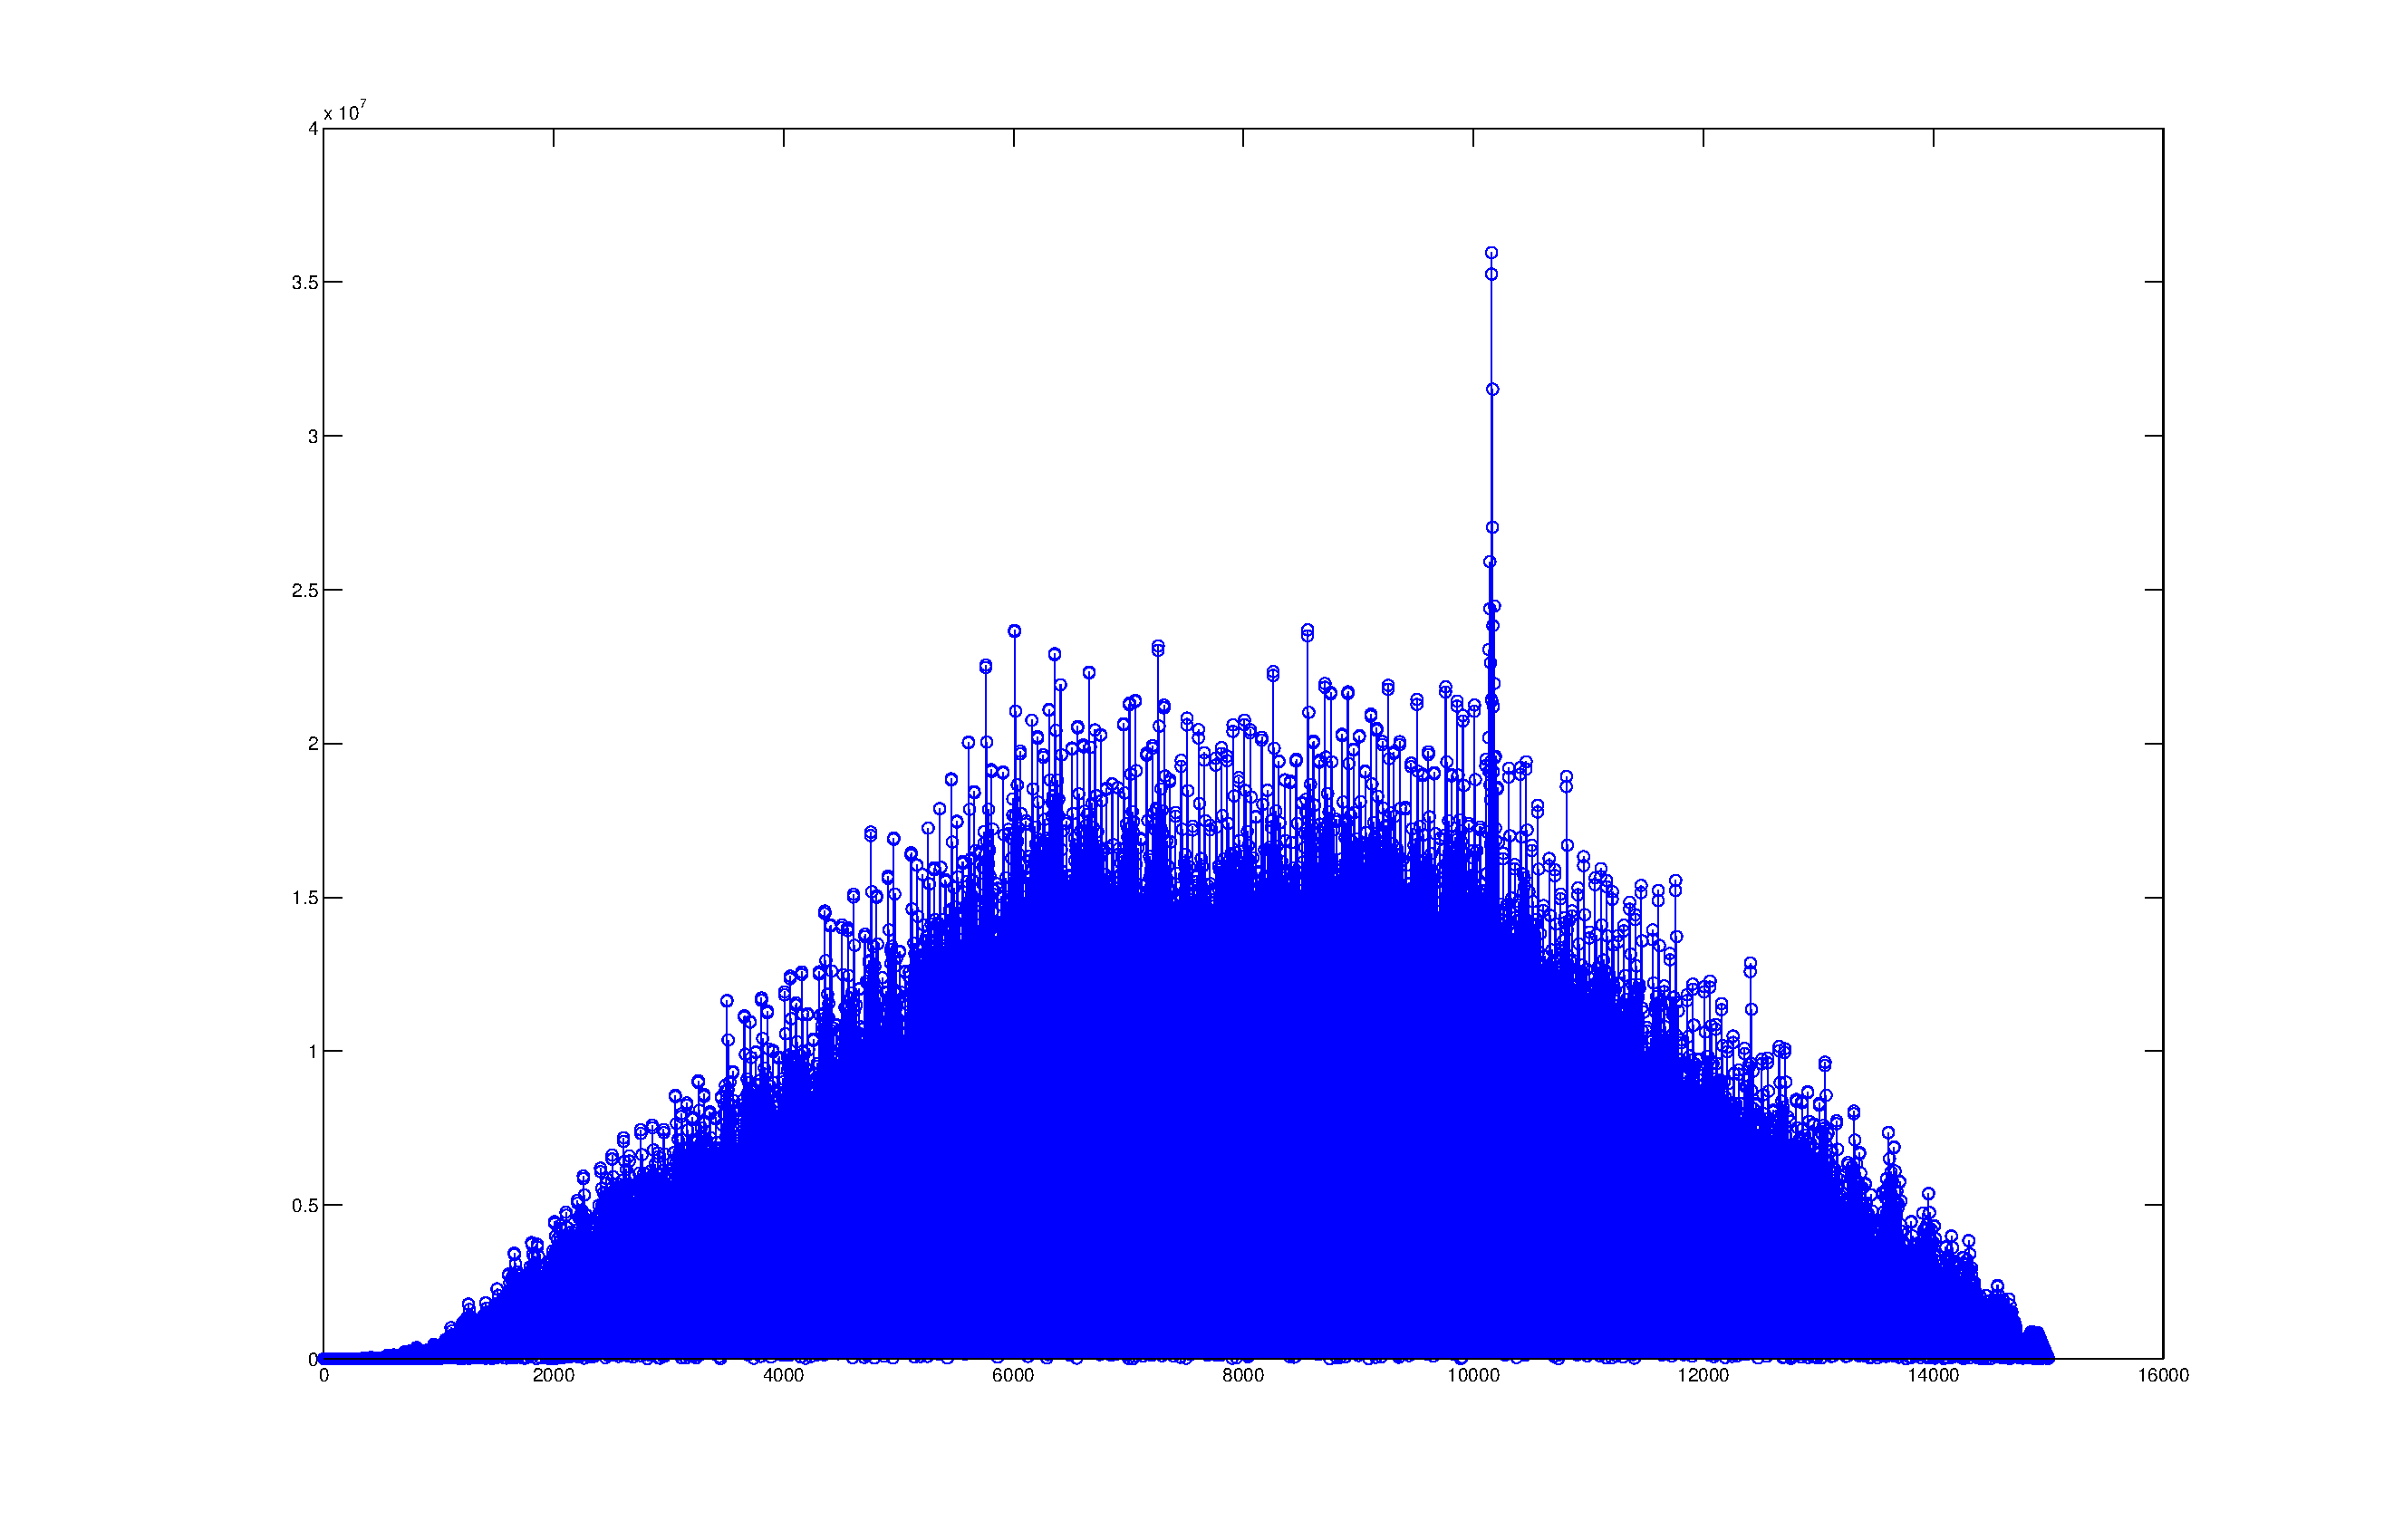
\includegraphics[width=1\linewidth]{100eq.eps} 
    \caption{One sample resolution cross correlation with training sequence of length 100 symbols and equal frequency to rest of trasmission.} 
    \label{fig7:c} 
  \end{subfigure}%%
  \quad
  \begin{subfigure}[b]{0.5\linewidth}
    \centering
    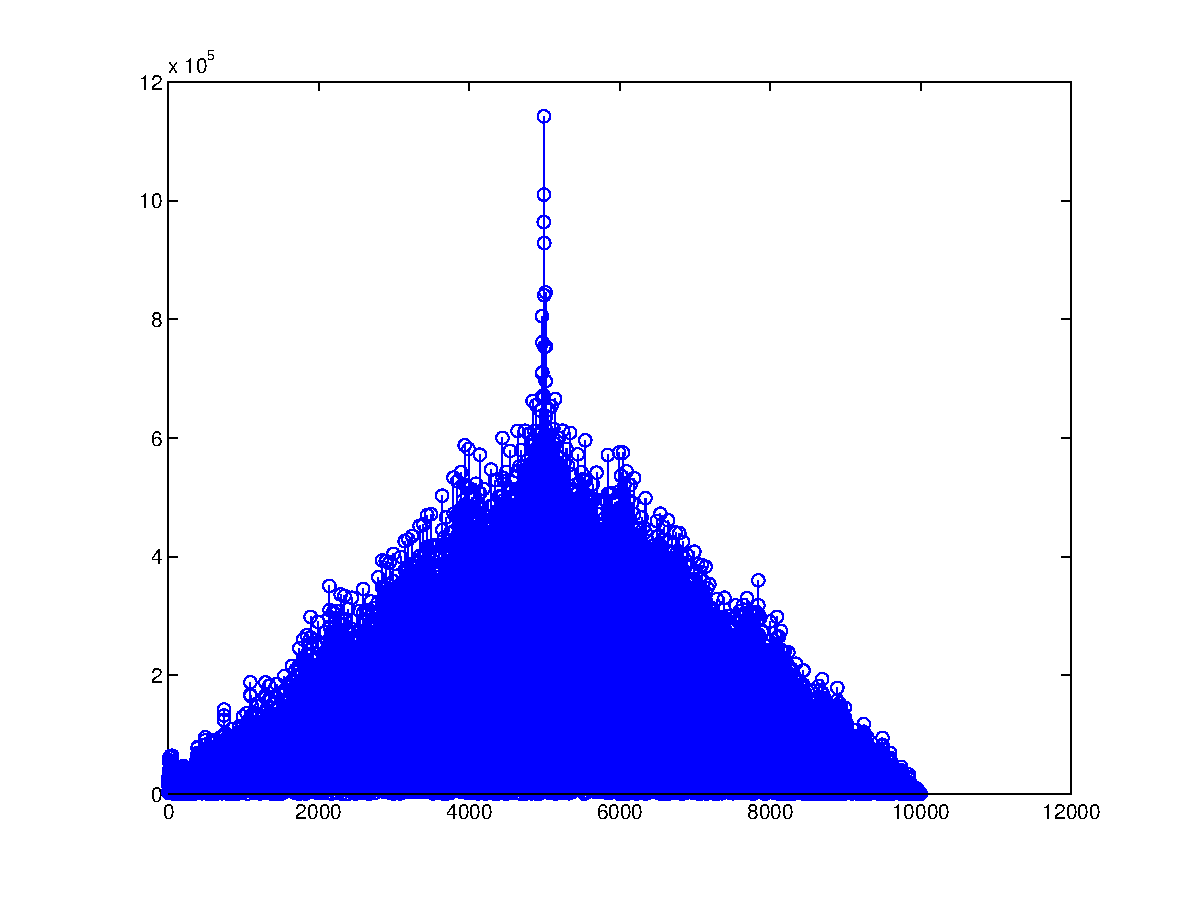
\includegraphics[width=1\linewidth]{100dif.eps} 
    \caption{One sample resolution cross correlation with training sequence of length 100 symbols and different frequency to rest of transmission.} 
    \label{fig7:d} 
  \end{subfigure} 
  \caption{Training sequence algorithm/length/modulation comparison.}
  \label{tscomp} 
\end{figure}
   
\subsubsection{Carrier Synchronisation}

The basic operations required by an all digital MQAM receiver is illustrated in figure \ref{rxMQAM}. The quadrature down-conversion and matched filter operations produce estimates of the quadrature amplitudes that are the basis of the data decisions. The role of carrier phase synchronisation is to perform the quadrature down-conversion using phase coherent replicas of the quadrature carriers.

 \begin{figure}[h]
  \centering
    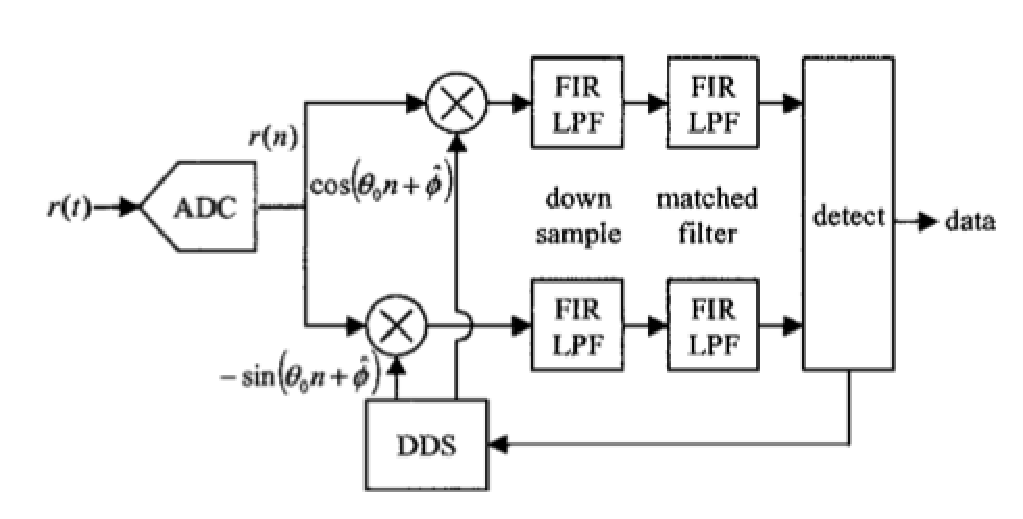
\includegraphics[width=0.6\textwidth]{rxMQAM.pdf}
    \caption{Block diagram of basic QPSK/QAM digital receiver. In the digital implementation, the VCO takes the form of a direct digital synthesizer (DDS). }
    \label{rxMQAM}
\end{figure}

There are many options for implementing carrier phase and frequency synchronisation in a digital communication system. At the heart of all synchronisers is the phase-locked loop (PLL). An all-digital receiver can be implemented with a digital phase-locked loop (DPLL) as shown in figure \ref{DPLL}. The phase detector is implemented using the arctangent suggested by the ATAN block. The complexity of the phase detector can be reduced by computing a signal proportional to the sine of the phase difference. The phase error is computed by comparing the phase difference between the received signal $x(n) + jy(n)$ and the closest constellation point $\hat{I}(n) + j\hat{Q(n)}$ as illustrated in figure \ref{PD}.

 \begin{figure}[h]
 \centering
\begin{subfigure}{0.5\textwidth}
 \centering
    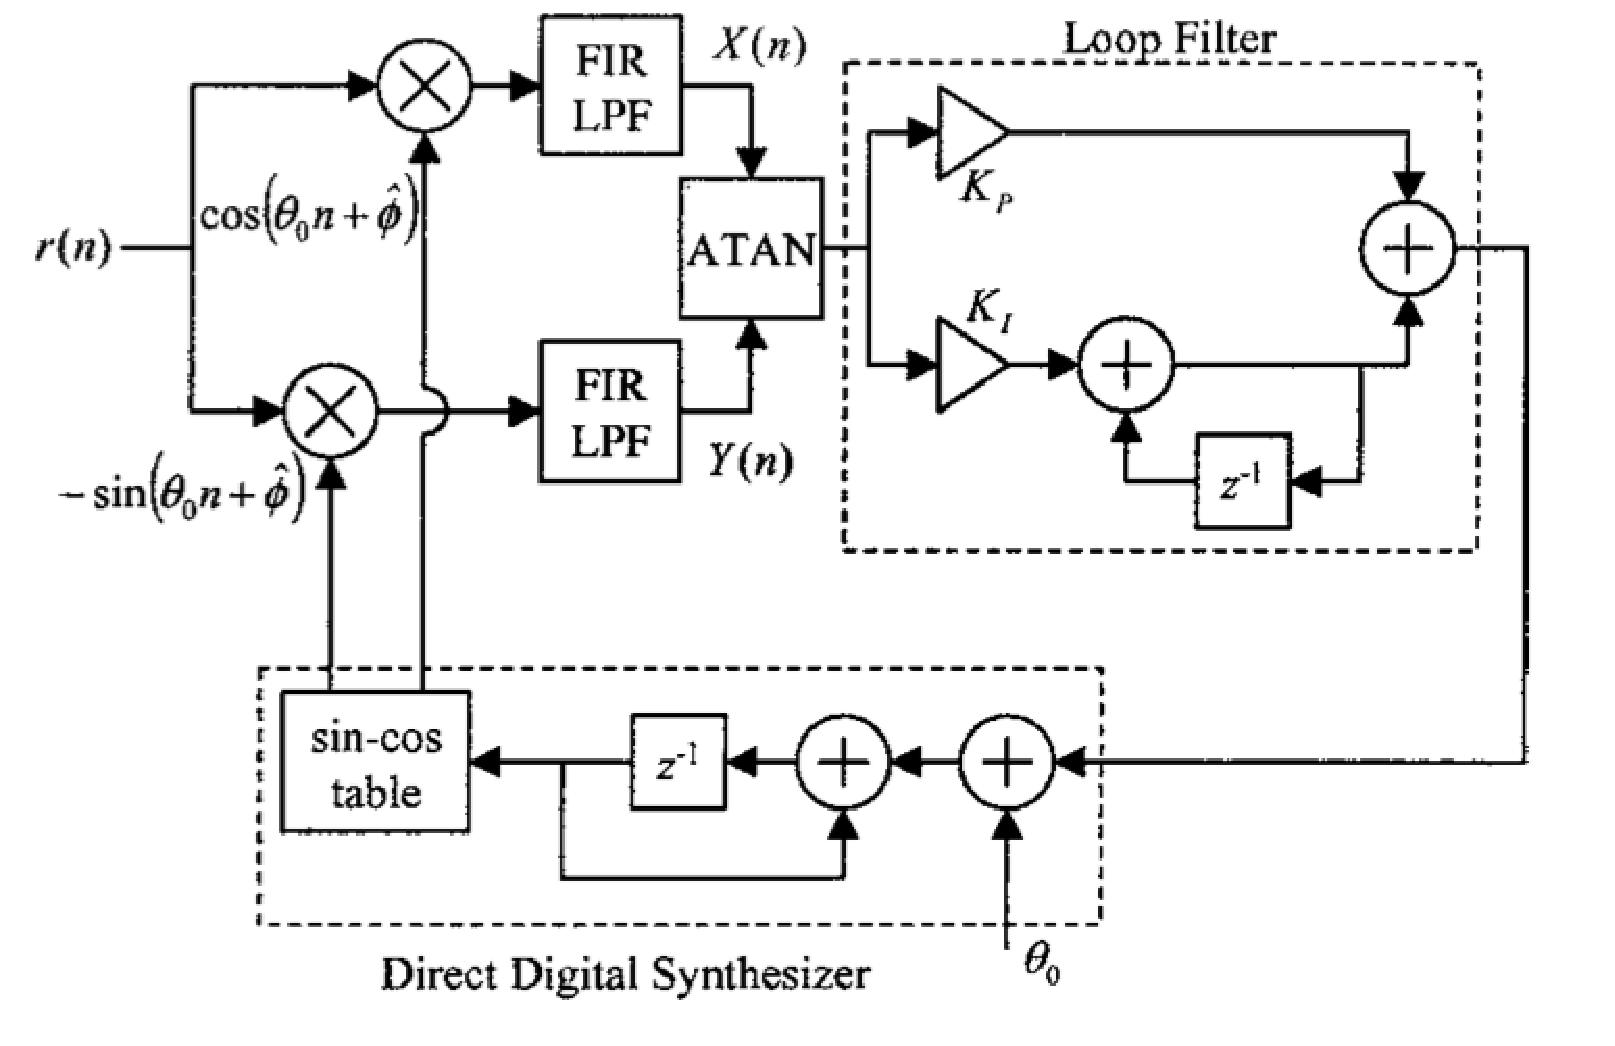
\includegraphics[width=0.9\linewidth]{DPLL.pdf}
    \caption{Digital phase locked loop for carrier phase synchronisation.}
    \label{DPLL}
\end{subfigure}%
\begin{subfigure}{0.5\textwidth}
 \centering
    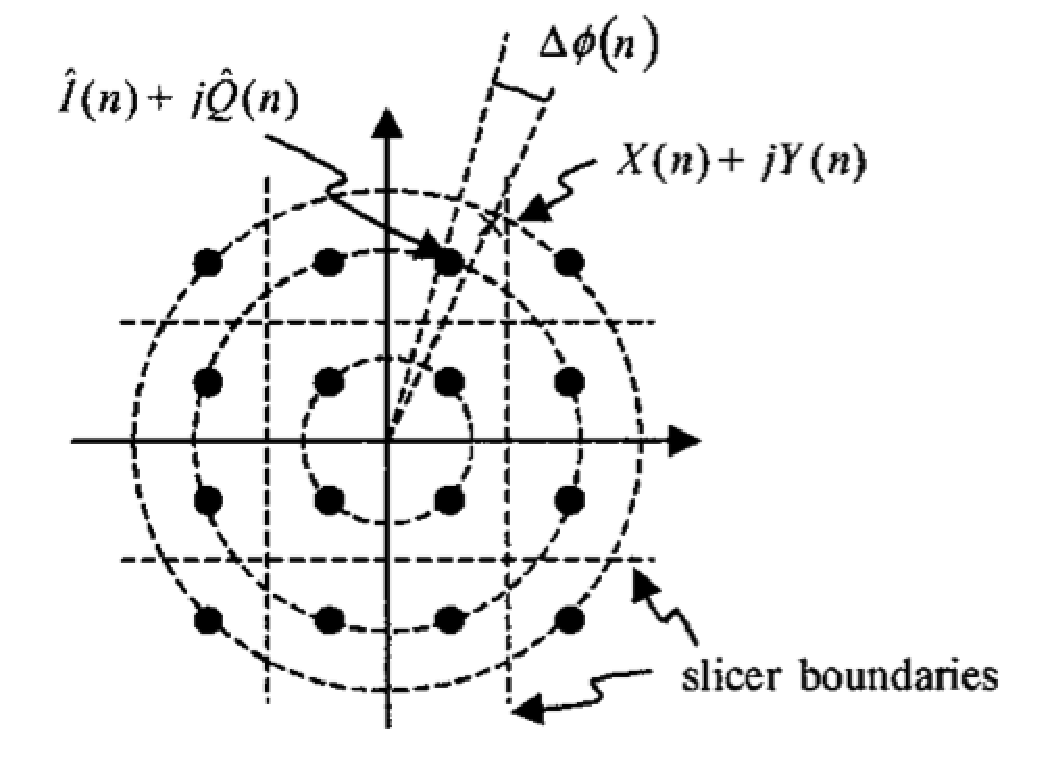
\includegraphics[width=0.7\linewidth]{PD.pdf}
    \caption{16-QAM constellation with decision boundaries and phase error.}
    \label{PD}
    \end{subfigure}
    \caption{Carrier phase estimation diagrams.}
    \label{carrierphase}
\end{figure}



The initial phase estimation can be done using the above procedure, taking into account the training sequence is known at transmitter and receiver. Let's assume the channel causes a rotation of $\varphi$ to the symbol constellation. The value of $\varphi$ can be computed using the element-wise multiplication of the received symbol with the complex conjugate of a modulated training sequence replica and then averaging over the sequence. In other words, if ${\left\{ {\tilde r(n)} \right\}_{n = 0}^{L - 1}}$ denotes the L received symbols and ${\left\{ {c(n)} \right\}_{n = 0}^{L - 1}}$ the local replica of the complex training sequence, an estimate of the phase offset can be obtained as:
\[\hat \varphi  = \frac{1}{L}\sum\limits_{k=0}^{L - 1} {\arg (\tilde r(k)c(k)^*)} \]
The longer the training sequence, the better the phase estimate as the influence from the noise decreases. A long training sequence, on the other hand, reduces the amount of payload that can be transmitted during a given time.

Another problem that may be faced in a real implementation is the Doppler shift introduced during the transmission, which causes the constellation to rotate further more (than the initial rotation). This frequency offset could be the result of relative motion between the transmitter and receiver, as would be the case with a mobile terminal traveling away or towards a receiver. It could also be attributed to small frequency variations of the various synthesisers in both the transmitter and receiver, which are functions of time and temperature. In order to overcome this problem, at least two approaches are possible. The first is to introduce a training sequence in the data so that a new phase estimation can be computed, resulting in a lower rate. The other solution is to divide the decisions into various small blocks in which the offset does not influence the decision, estimate the phase rotation from the nearest points and rotate the constellation for future decisions. In this way the rate is not affected but a correct decision in each block is assumed. The frequency offset effect can be seen in figure \ref{phaseoff}, where a signal of 5 seconds was transmitted. The second solution was used to correct the phase with great success.


 \begin{figure}[h]
 \centering
\begin{subfigure}{0.32\textwidth}
 \centering
    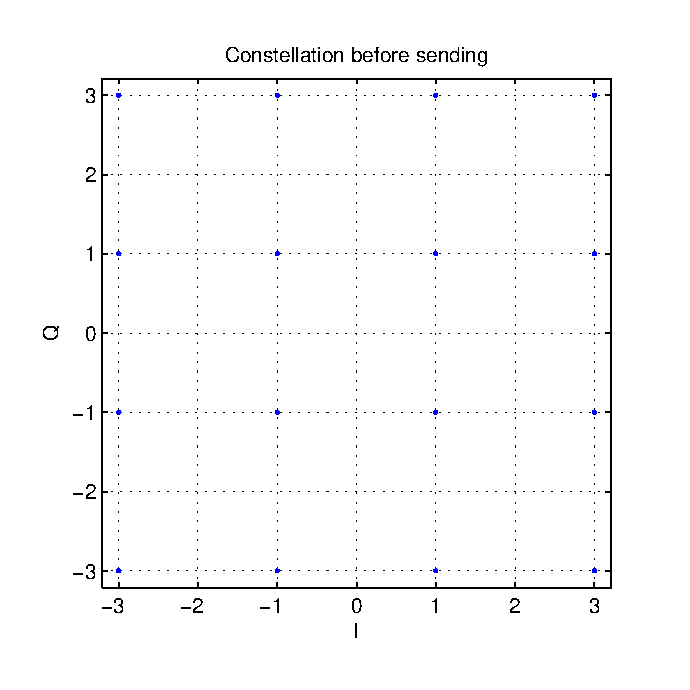
\includegraphics[width=0.8\linewidth]{tx_const.eps}
    \caption{Transmitted constellation.}
    \label{DPLL}
\end{subfigure}%
\begin{subfigure}{0.32\textwidth}
 \centering
    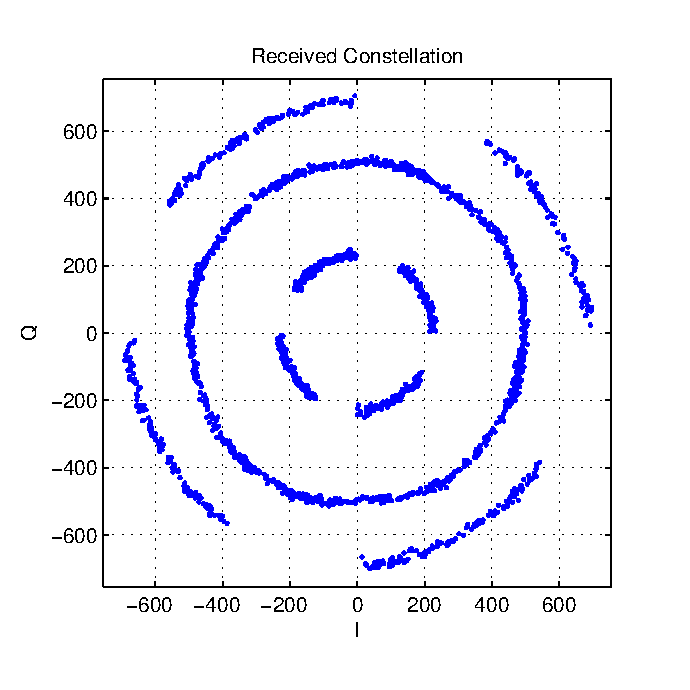
\includegraphics[width=0.8\linewidth]{rx_const.eps}
    \caption{Received constellation.}
    \label{PD}
    \end{subfigure}
    \begin{subfigure}{0.32\textwidth}
 \centering
    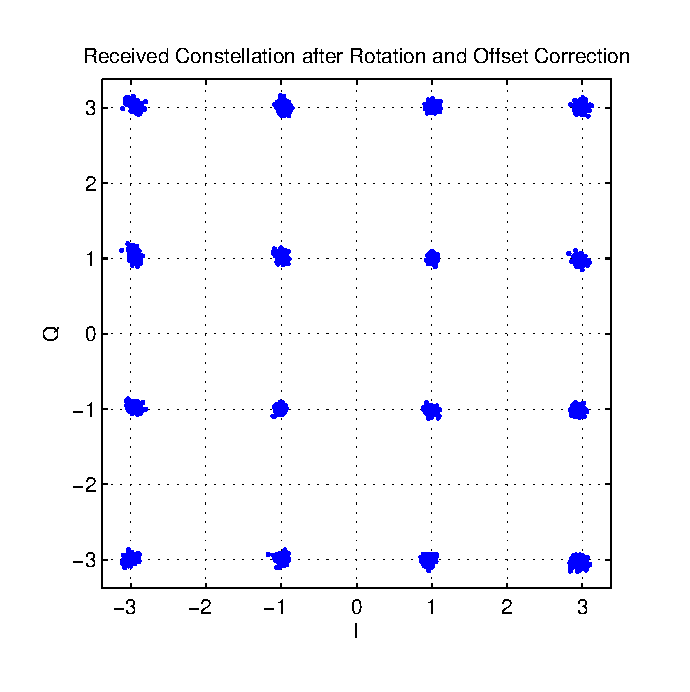
\includegraphics[width=0.8\linewidth]{rx_const_after.eps}
    \caption{Received constellation after phase correction.}
    \label{PD}
    \end{subfigure}
    \caption{Example of frequency offset in a 16-QAM constellation with decision boundaries.  }
    \label{phaseoff}
\end{figure}

%By trying different time-shifts in steps of $\frac{T}{Q}$, where Q is the number of samples per symbol, the symbol timing can be found with a resolution of  $\frac{T}{Q}$.  

\clearpage

\section{Android part}

Used Software and Hardware \\

1. MATLAB R2013a \\
2. Eclipse with SDK version 3.8.0 \\
3. ADT (Android development toolkit) \\
4.Samsung Galaxy S3 \\
5. Dell PCs with operating system Windows 7 and Mac with operating system OSx Mavericks \\


\subsection{FrameWork}

Martin Ohlsson developed an android code based workspace called FrameWork. FrameWork was the groundwork for our project and our following application. The file contained functions enabling initiation of variant sensor parts of the android phone (e.g. microphone, camera, gps etc.). Even thought some of the coding is irrelevant in out case, the file is containing everything needed as basis for our application development.
 \textcolor{red}{\subsection{PictureOfFrameWork}}

\subsection{Transmitter and Receiver}

Since we are transmitting and receiving a file through a 3,5mm cable we used two phones, one to transmit the file and the other to receive it. When starting the application, \textcolor{red}{four alternatives are given (change if we change layout)}. The user can kill the app, go in to transmitter mode or go in to receiver mode. The fourth option is to select a file, where the user selects the file to be transmitted. 


\clearpage

\begin{thebibliography}{1}

\bibitem{Madhow}
Upamanyu Madhow, \emph{Fundamentals of Digital Communication}, Cambridge , 2008

\bibitem{Proakis}
John G. Proakis, Masoud Salehi, \emph{Digital Communications}, McGraw-Hill , 2008

\end{thebibliography}


\end{document}
